\chapter{Results and Evaluation}
\label{chap:results-and-evaluation}

\section{DFT Data Convergence}

The quality of the DFT training data depends on the underlying approximations
and numerical details. While the overall accuracy depends mostly on the used
exchange-correlation functional, in this case the standard PBE, the precision
depends on multiple numerical parameters. If those are not converged, the
results can suffer from significant numerical noise or other undesired
effects, e.g., Pulay forces originating in the incompleteness of the basis
set. Therefore, a thorough check of the convergence of the relevant quantities
with respect to the crucial numerical parameters such as the $k$-point grid or
the energy cutoff is required.

We can clearly see from the energy cutoff convergence plot
(figure \ref{fig:dft_energy_cutoff_convergence}) that the energy errors due
to numerical approximations are on the order of $100 \, \mathrm{meV}$,
dividing by the number of atoms, we get an error of an order of
$1 \, \mathrm{meV}$. The force errors due to numerical approximations are on
the order of $10^{-5} \, \mathrm{eV}/\text{\AA}$. The $k$-point convergence
plot (figure \ref{fig:dft_kpoint_convergence}) shows that the energy errors
due to numerical approximation are on the order of $1 \, \mathrm{meV}$,
dividing by the number of atoms, we get an error of an order of
$10^{-2} \, \mathrm{meV}$. The force errors due to numerical approximation are
on the order of $10^{-4} \, \mathrm{eV}/\text{\AA}$. This means that our DNN
model should ideally give energy predictions with an error of order
$10^{-1} \, \mathrm{meV}$ and force predictions with an error of order
$10^{-4} \, \mathrm{eV}/\text{\AA}$. Errors above these magnitudes are
most likely not caused by the numerical approximations of the DFT data or the
accuracy of the simulation algorithms chosen. It's also very important to note
that the average forces are very close to zero.

\begin{figure}
  \begin{center}
    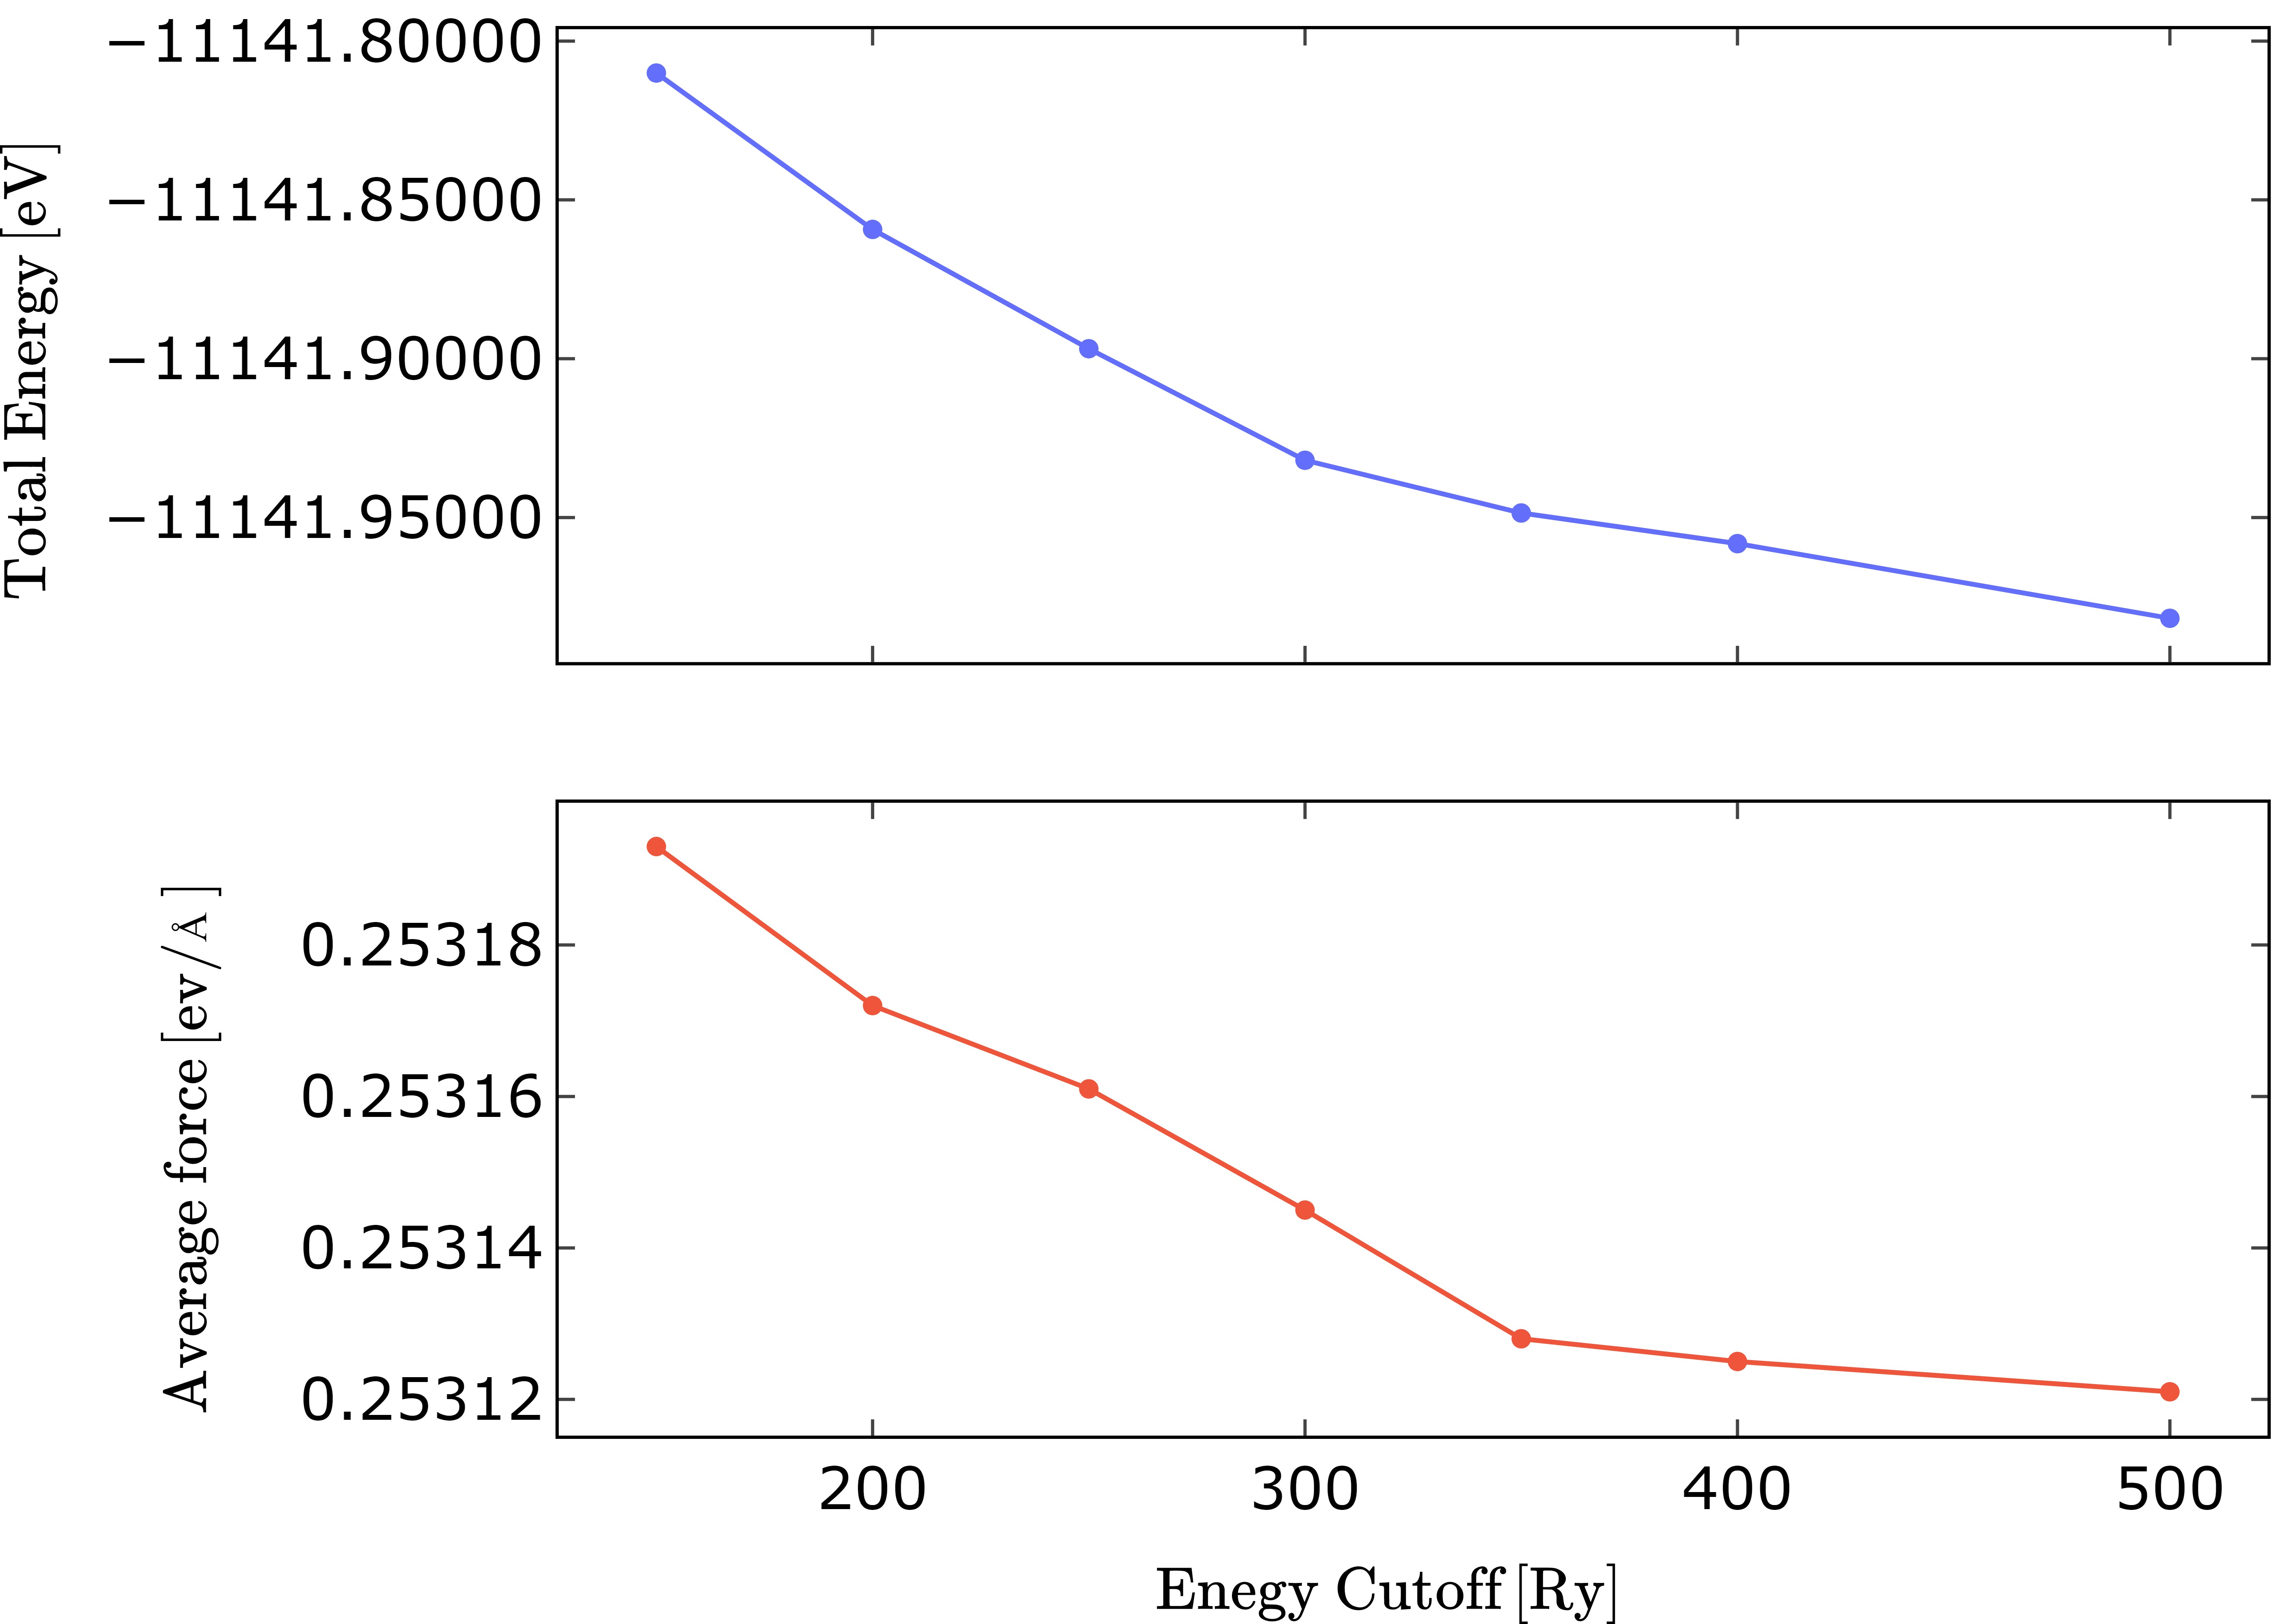
\includegraphics[width=.8\textwidth]{
      asset/cutoff_convergence.jpg
    }
  \end{center}
  \caption{Energy cutoff convergence test for the DFT training data.}
  \label{fig:dft_energy_cutoff_convergence}
\end{figure}

\begin{figure}
  \begin{center}
    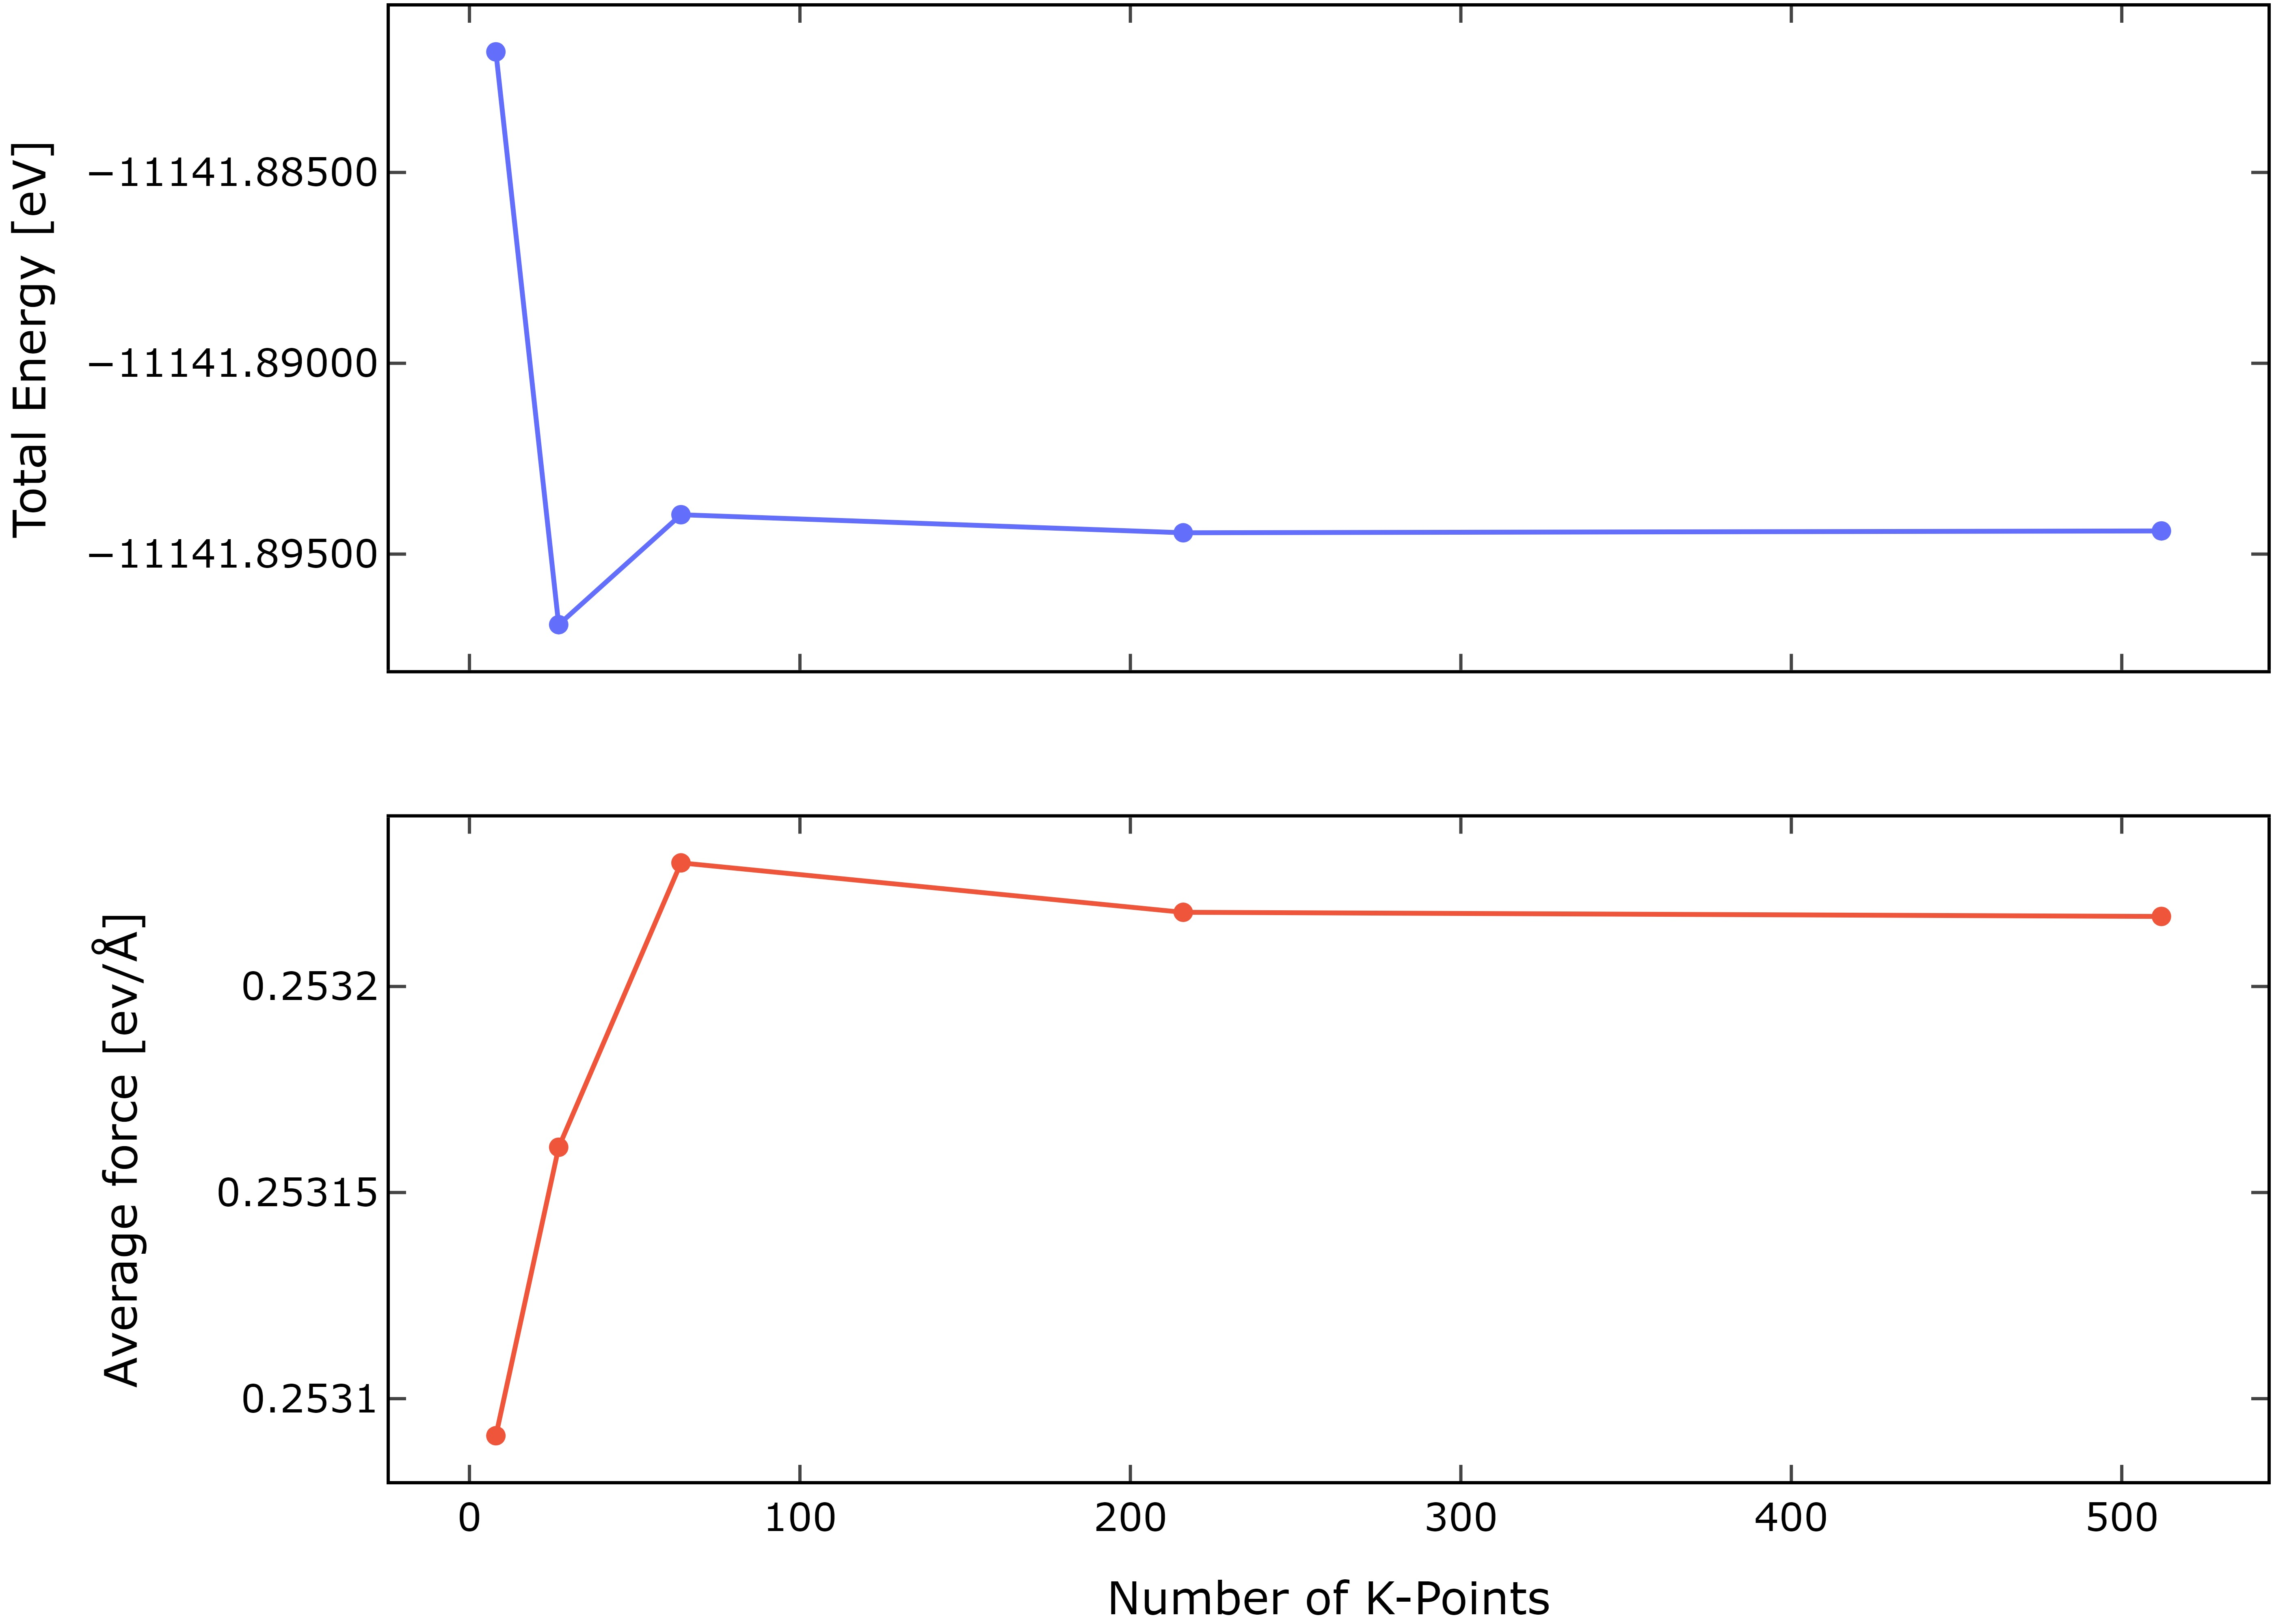
\includegraphics[width=.8\textwidth]{
      asset/kpoint_convergence.jpg
    }
  \end{center}
  \caption{$k$-point convergence test for the DFT training data.}
  \label{fig:dft_kpoint_convergence}
\end{figure}

\section{Training Results}

All models were trained on a dual AMD EPYC 7H12 64-Core processor machine.
Although such specs look impressive, the underlying training algorithms used
by DeepMD-kit seem to not be optimized for CPU training, and the whole process
could probably be greatly accelerated by training on GPUs. DeepMD-kit allows
you to fine-tune the training process by adjusting the runtime parameters
\texttt{OMP\_NUM\_THREADS}, \texttt{TF\_INTRA\_OP\_PARALLELISM\_THREADS},
and \texttt{TF\_INTER\_OP\_PARALLELISM\_\allowbreak{}THREADS}. Despite running
many empirical tests to arrive at the optimal values for these parameters, the
training process did not speed up significantly. The training sessions took
about $12 \, \mathrm{h}$ for the larger models and about $8 \, \mathrm{h}$ for
the smaller models.

A typical descending learning curve was observed for models trained on the
amorphous and combined datasets. When increasing the number of descriptor
neurons from $[5, 10, 20]$ (figure
\ref{fig:amorphous_5,10,20d_20,20,20f_260222622s-learning-curves}) to
$[25, 50, 100]$ (figure
\ref{fig:amorphous_25,50,100d_20,20,20f_260222622s-learning-curves}) we don't
observe significant changes in the learning curves. On the other hand, when
increasing the number of fitting neurons from $[10, 10, 10]$
(figure \ref{fig:amorphous_10,20,40d_10,10,10f_260222622s-learning-curves}) to
$[75, 75, 75]$ (figure
\ref{fig:amorphous_10,20,40d_75,75,75f_260222622s-learning-curves}) we can
observe a very slight divergence of training error and validation error with
increasing training steps. We can see from the error evaluation plot for
descriptor neurons (figure \ref{fig:descriptor_energy_error_evaluation}) that
the energy error slightly decreases with increasing number of descriptor
neurons, although this effect is negligible. This is expected, i.e., a larger
number of parameters in general leads to a better fit. The effect of
increasing energy error with increasing number of fitting neurons can also be
observed in the error evaluation plot for fitting neurons (figure
\ref{fig:fitting_energy_error_evaluation}). Both of these effects are much
more pronounced for the crystalline dataset, where data scarcity is a
significant concern. Although the crystalline system should be the simplest
to model, the shortage of data plays a major role here, which can be observed
in the learning curves and in the energy error evaluation plots. Too large
fitting network architectures for the crystalline set lead to overfitting,
i.e., there are too many free parameters for the available data and, the
training begins to fit the random noise in the data. In fact, this is the
reason why an independent validation dataset is used, as the large divergence
between the training and validation signals overfitting.
The predictions for the crystalline system get outstandingly better for both
the training and validation data when increasing the number of descriptor
neurons from $[5, 10, 20]$ (figure
\ref{fig:crystalline_5,10,20d_20,20,20f_260222622s-learning-curves}) to
$[25, 50, 100]$ (figure
\ref{fig:crystalline_25,50,100d_20,20,20f_260222622s-learning-curves}) for
both validation and training datasets. The higher number of descriptor
neurons allows the model to better capture the underlying structure of the
sillicon system, since this effect is observable for the amorphous and
combined systems as well. While the number of descriptor neurons in the tested
range correlates positively with inference quality, the opposite is true for
the number of fitting neurons. When increasing fitting neurons from
$[10, 10, 10]$
(figure \ref{fig:crystalline_10,20,40d_10,10,10f_260222622s-learning-curves})
to $[75, 75, 75]$
(figure \ref{fig:crystalline_10,20,40d_75,75,75f_260222622s-learning-curves})
we observe that the energy error increases and the dissonance between
training error and validation error broadens. In this case, the model
architecture is too complex and overfits on the small sample of training data.
We can also see the discussed effects in the error evaluation plots for
descriptor neurons and fitting neurons (figures
\ref{fig:descriptor_energy_error_evaluation} and
\ref{fig:fitting_energy_error_evaluation} respectively).

The force errors in all of the learning curves seem to converge relatively
quickly for all of the training sessions. Further training steps don't seem to
significantly improve the prediction quality and may even lead to worse
predictions. This is most likely due to the fact that the forces are very
close to zero for most of the training data, and the models are able to learn
the small deviations from zero very quickly. The increase in force error over
time is caused by the fact that the weights of the objective function are
initially set to prioritize the force error over the energy error and then
gradually shift towards prioritizing energy error over force error, as already
discussed.

\begin{figure}
  \begin{center}
    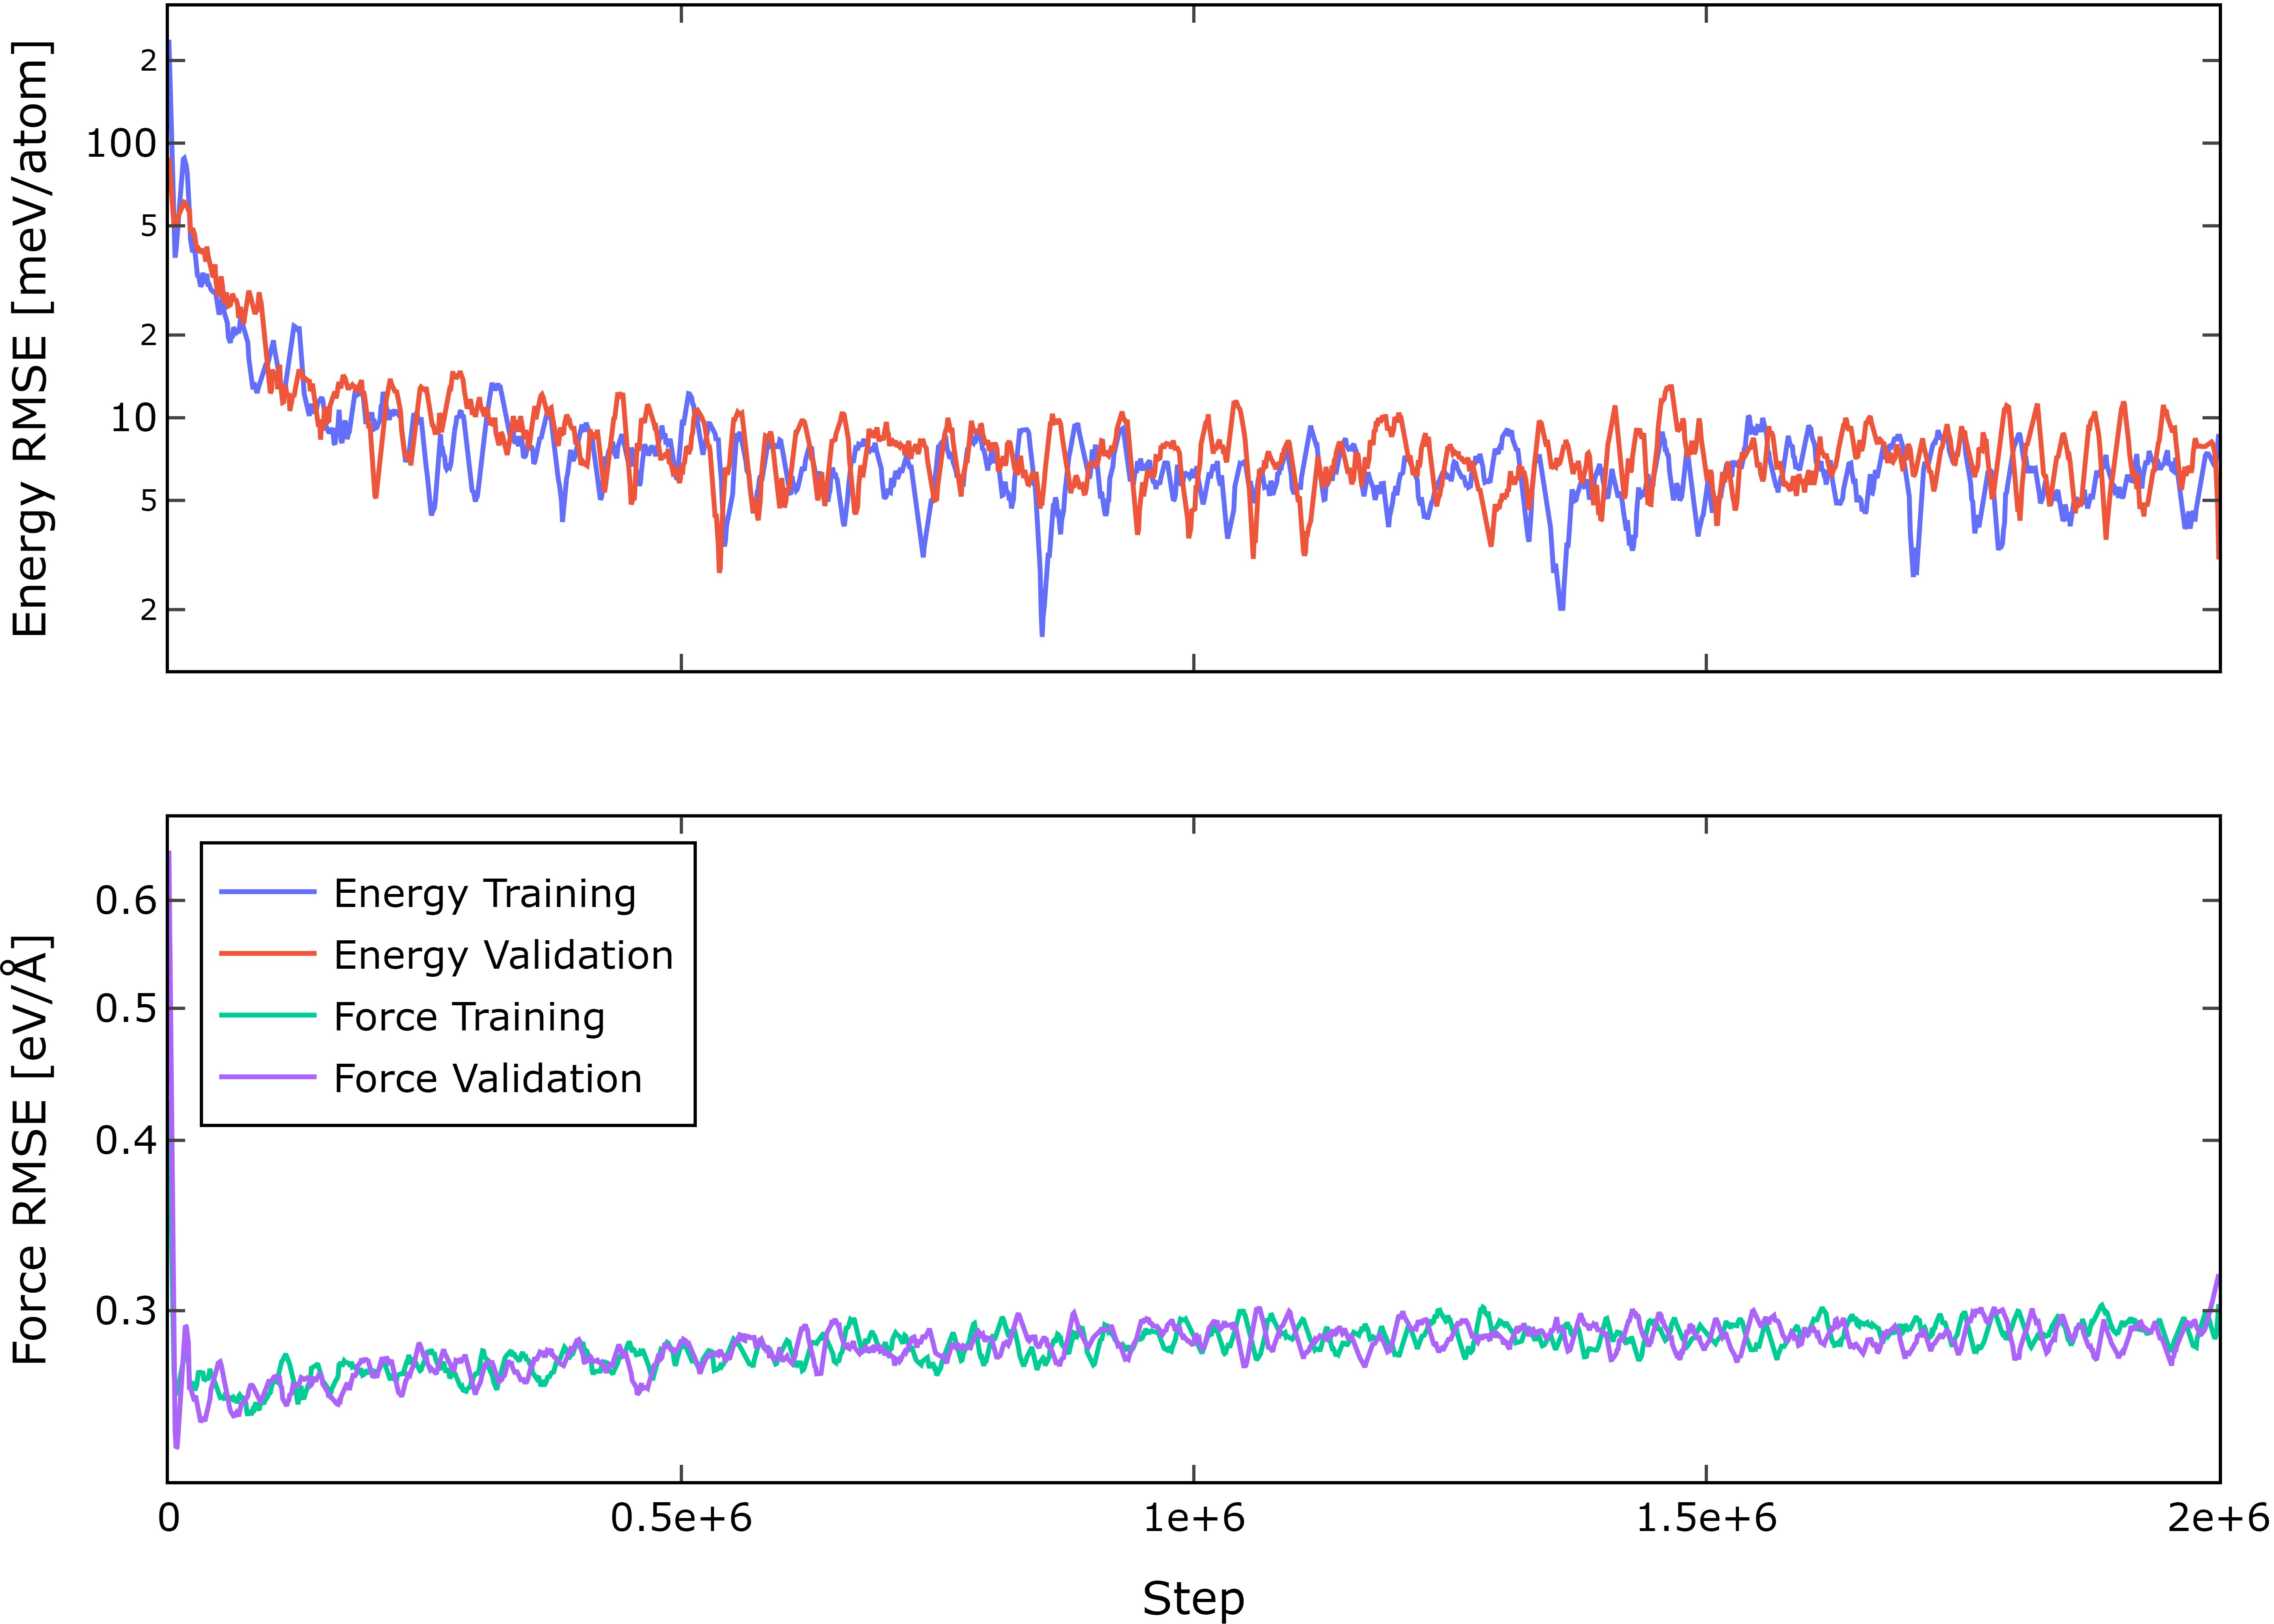
\includegraphics[width=.8\textwidth]{
      asset/amorphous_5,10,20d_20,20,20f_260222622s_energy_force_l_curve.jpg
    }
  \end{center}
  \caption{Learning curves for model \texttt{amorphous\_5,10,20d\_20,20,\allowbreak{}20f\_260222622s}.}
  \label{fig:amorphous_5,10,20d_20,20,20f_260222622s-learning-curves}
\end{figure}

\begin{figure}
  \begin{center}
    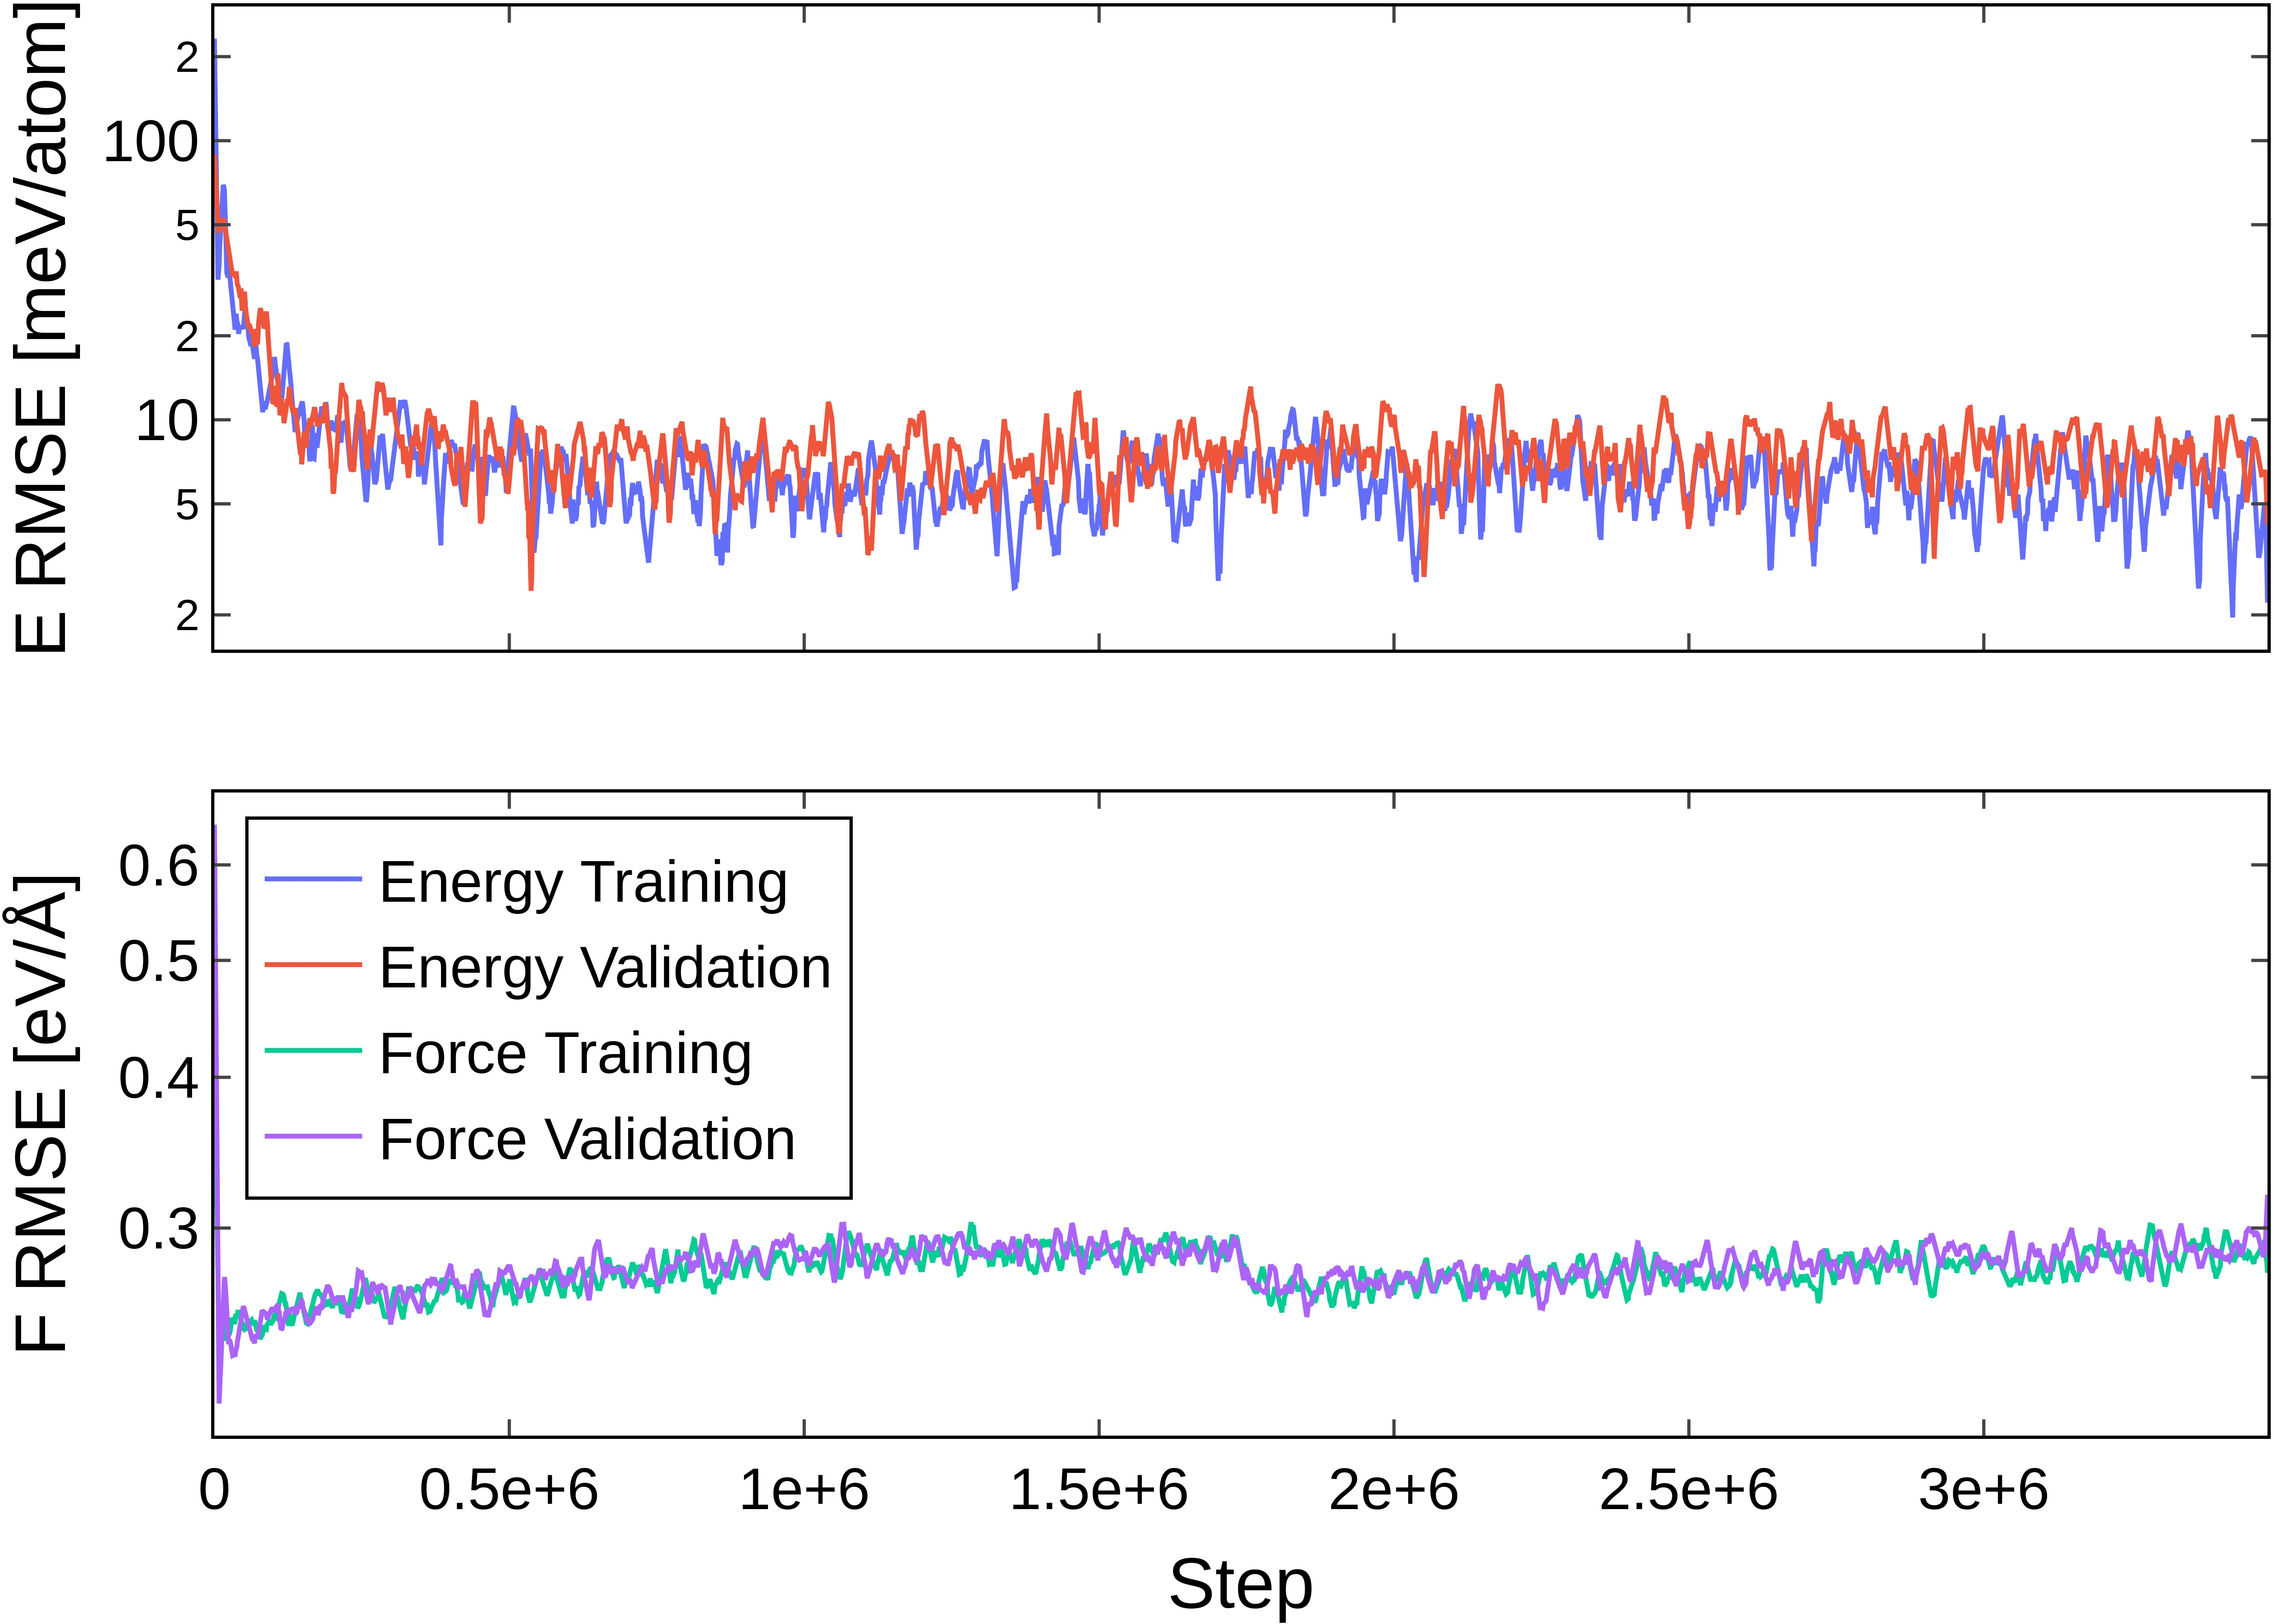
\includegraphics[width=.8\textwidth]{
      asset/amorphous_25,50,100d_20,20,20f_260222622s_energy_force_l_curve.jpg
    }
  \end{center}
  \caption{Learning curves for model \texttt{amorphous\_25,50,100d\_20,20,\allowbreak{}20f\_260222622s}.}
  \label{fig:amorphous_25,50,100d_20,20,20f_260222622s-learning-curves}
\end{figure}


\begin{figure}
  \begin{center}
    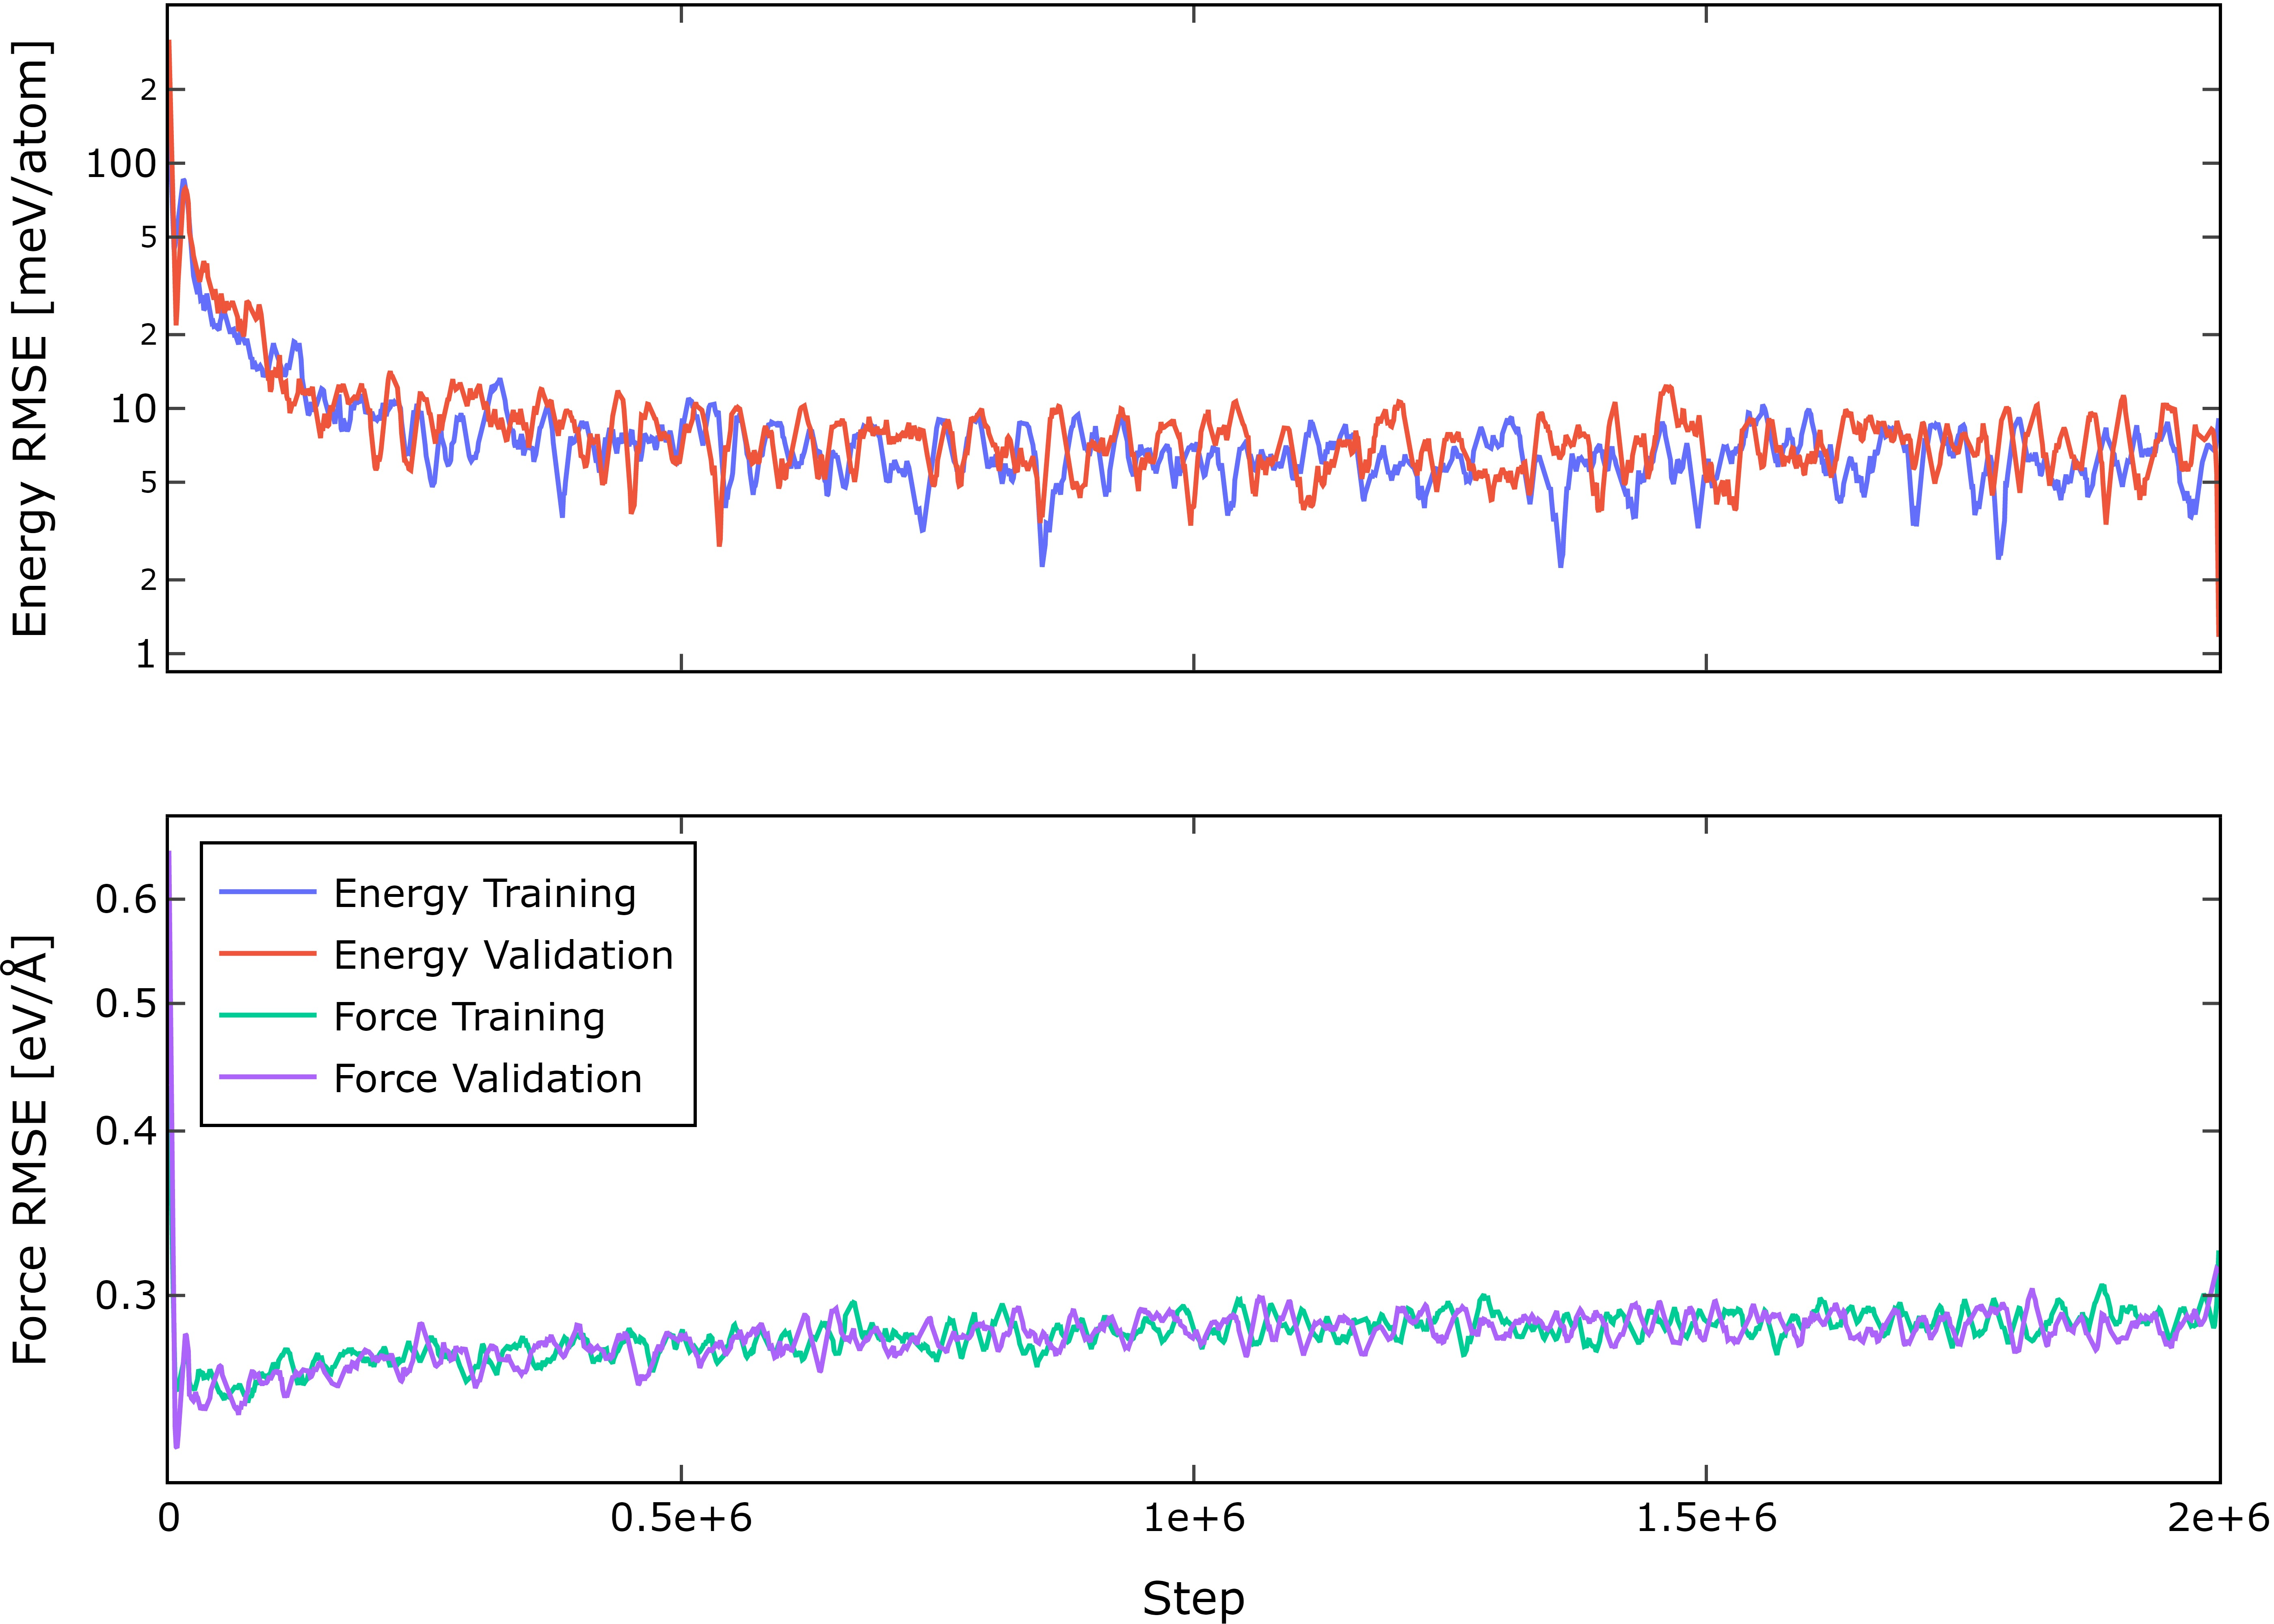
\includegraphics[width=.8\textwidth]{
      asset/amorphous_10,20,40d_10,10,10f_260222622s_energy_force_l_curve.jpg
    }
  \end{center}
  \caption{Learning curves for model \texttt{amorphous\_10,20,40d\_10,10,\allowbreak{}10f\_260222622s}.}
  \label{fig:amorphous_10,20,40d_10,10,10f_260222622s-learning-curves}
\end{figure}

\begin{figure}
  \begin{center}
    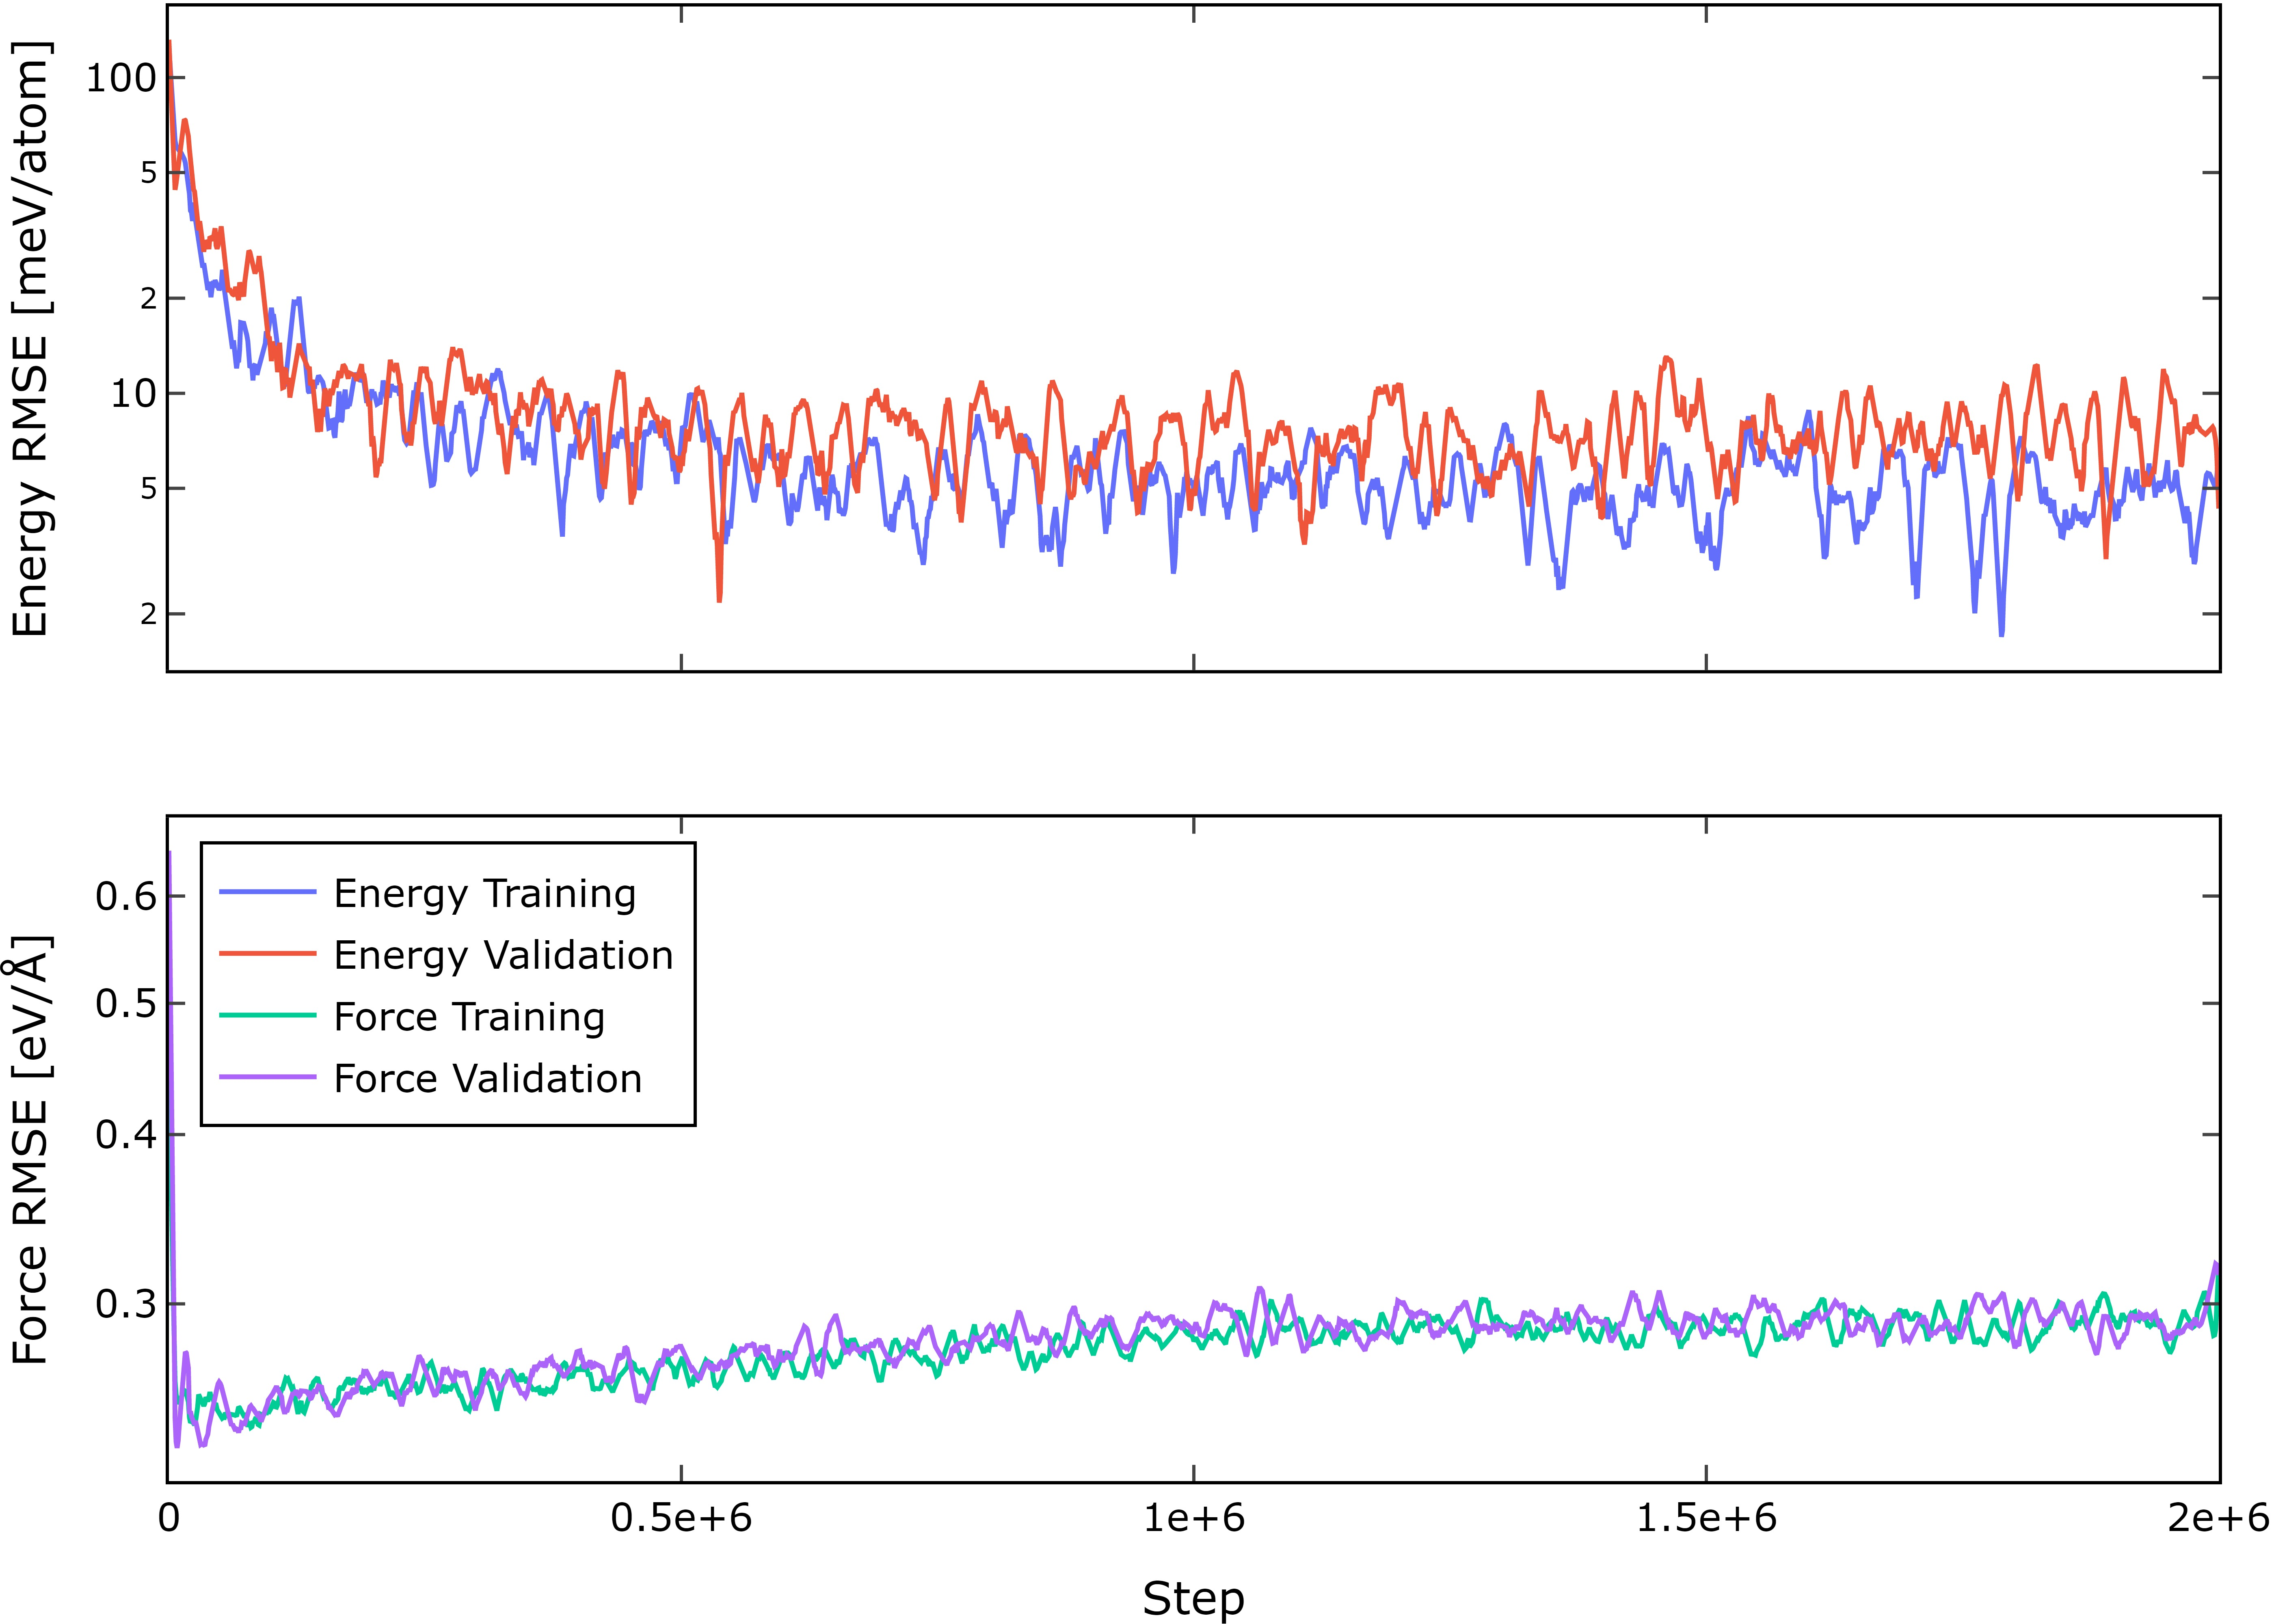
\includegraphics[width=.8\textwidth]{
      asset/amorphous_10,20,40d_75,75,75f_260222622s_energy_force_l_curve.jpg
    }
  \end{center}
  \caption{Learning curves for model \texttt{amorphous\_10,20,40d\_75,75,\allowbreak{}75f\_260222622s}.}
  \label{fig:amorphous_10,20,40d_75,75,75f_260222622s-learning-curves}
\end{figure}

\begin{figure}
  \begin{center}
    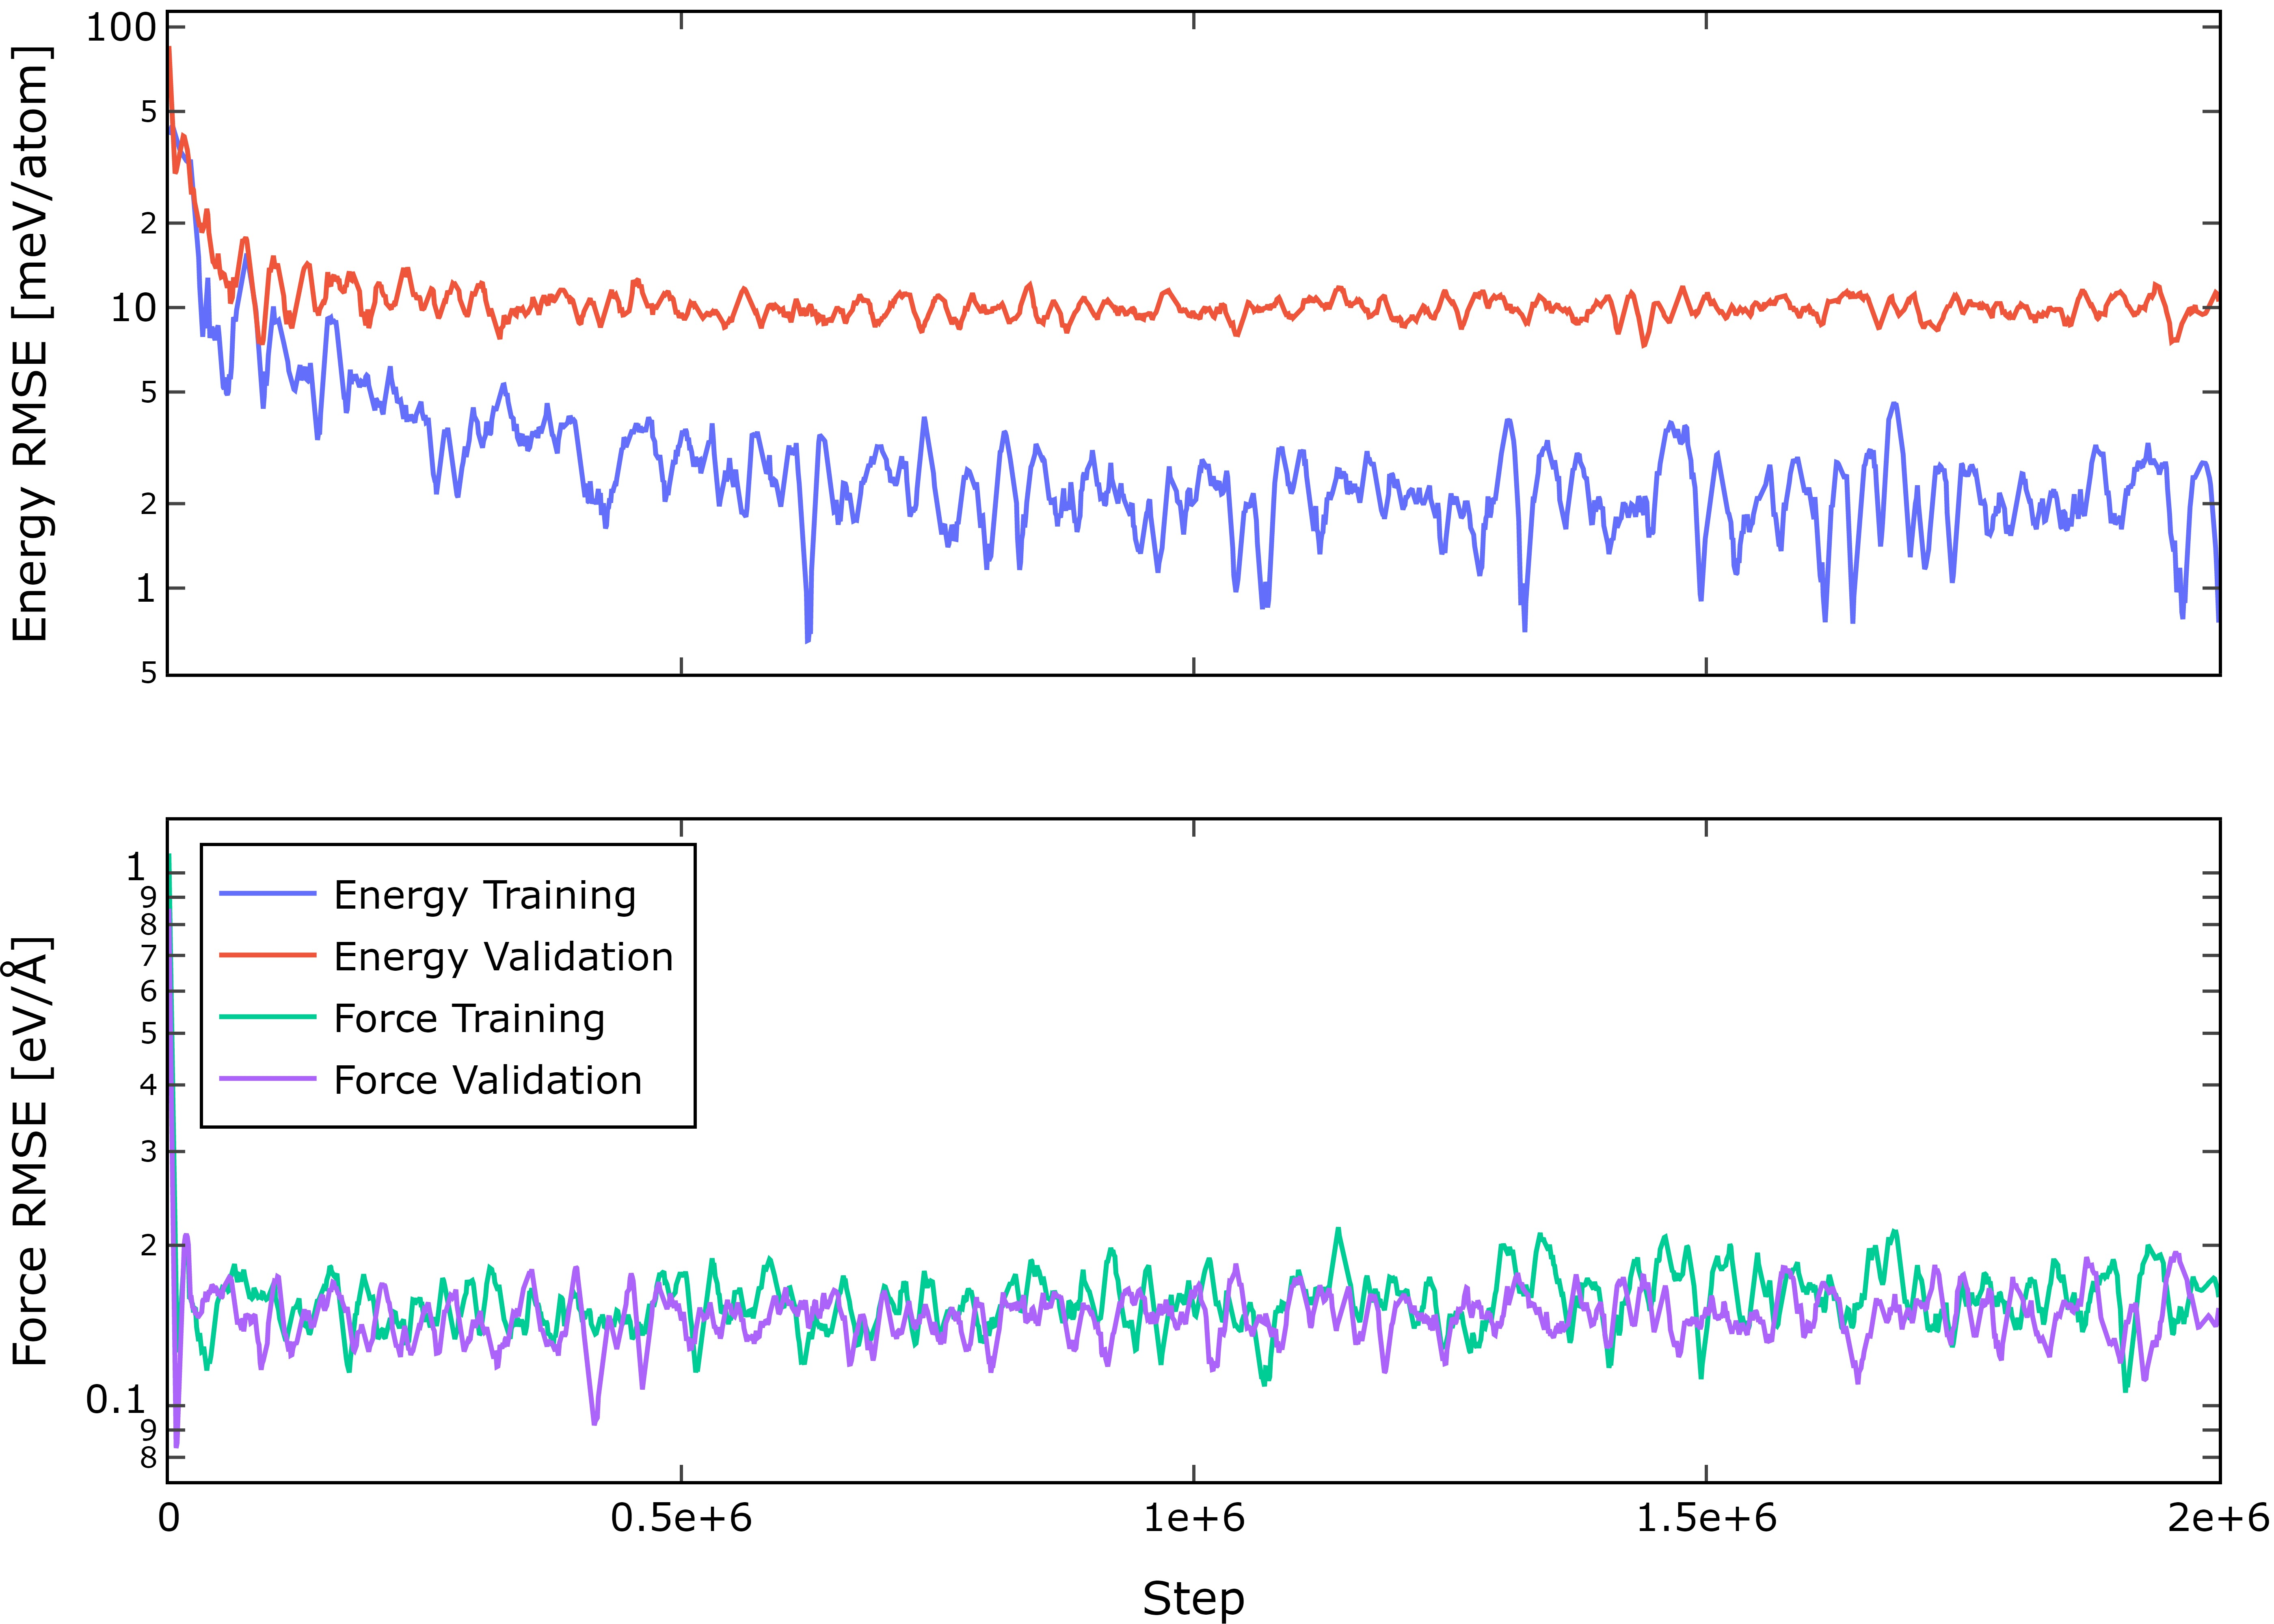
\includegraphics[width=.8\textwidth]{
      asset/crystalline_5,10,20d_20,20,20f_260222622s_energy_force_l_curve.jpg
    }
  \end{center}
  \caption{Learning curves for model \texttt{crystalline\_5,10,20d\_20,20,\allowbreak{}20f\_260222622s}.}
  \label{fig:crystalline_5,10,20d_20,20,20f_260222622s-learning-curves}
\end{figure}

\begin{figure}
  \begin{center}
    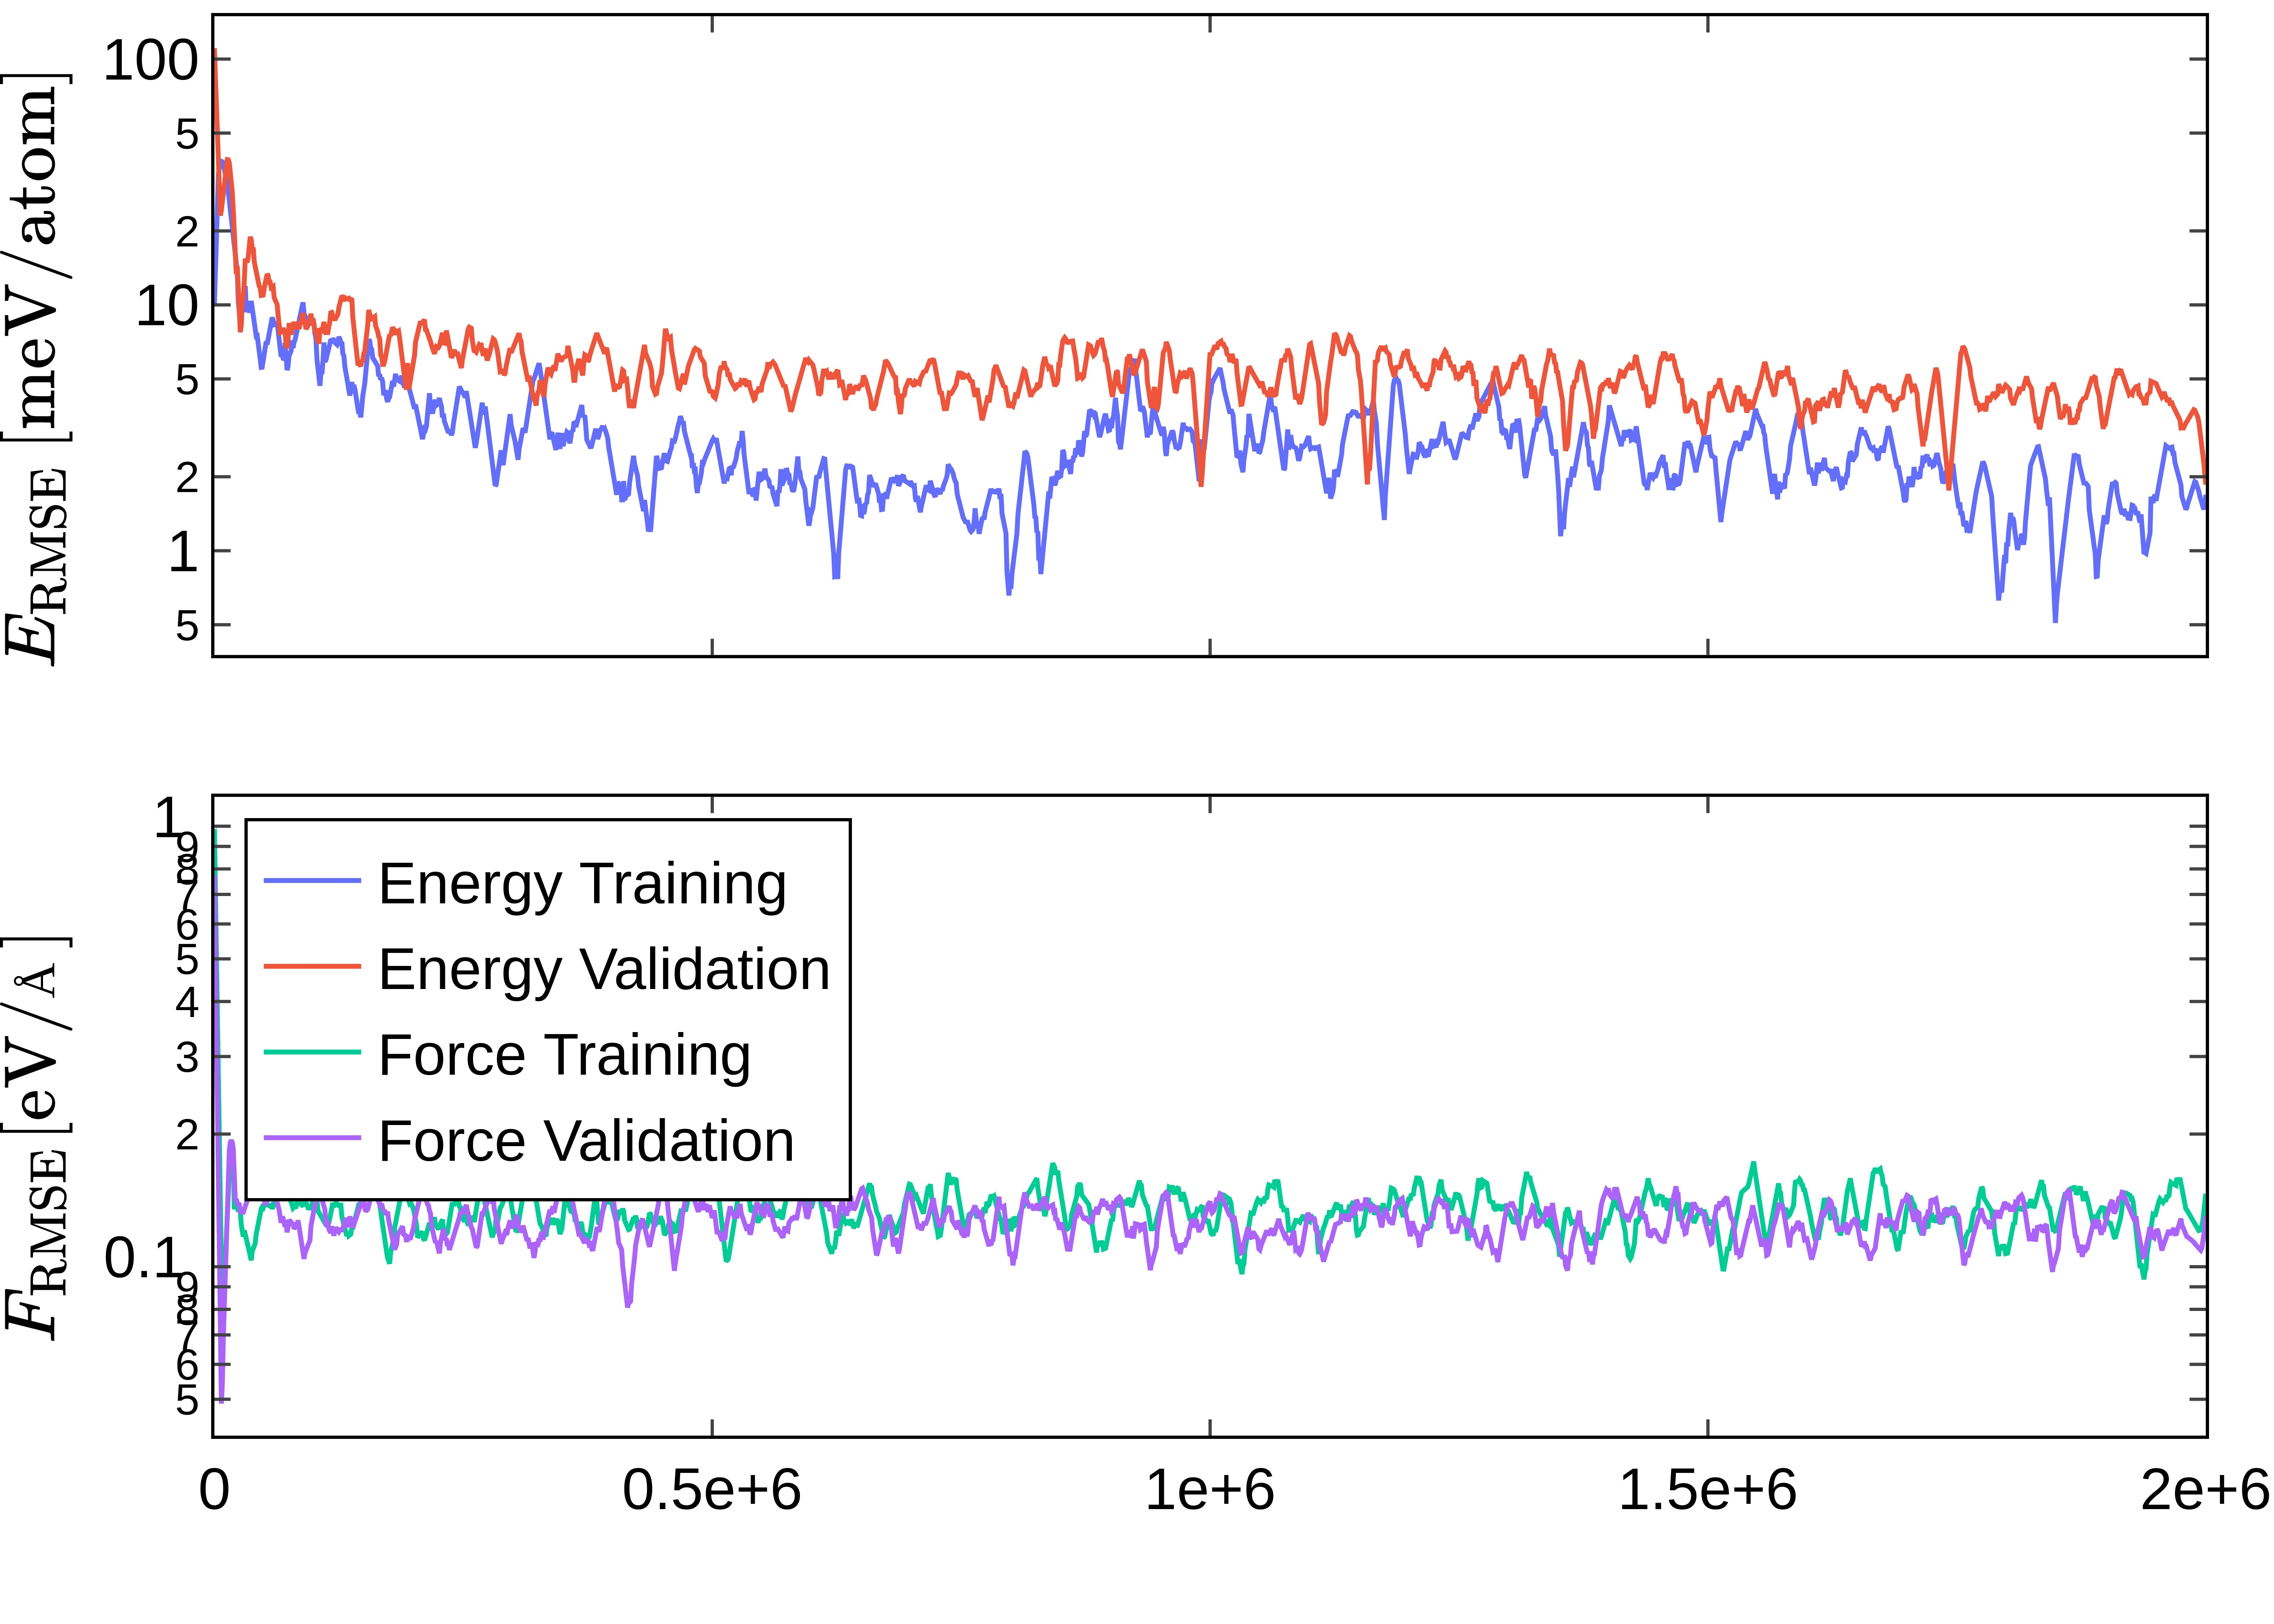
\includegraphics[width=.8\textwidth]{
      asset/crystalline_25,50,100d_20,20,20f_260222622s_energy_force_l_curve.jpg
    }
  \end{center}
  \caption{Learning curves for model \texttt{crystalline\_25,50,100d\_20,20,\allowbreak{}20f\_260222622s}.}
  \label{fig:crystalline_25,50,100d_20,20,20f_260222622s-learning-curves}
\end{figure}

\begin{figure}
  \begin{center}
    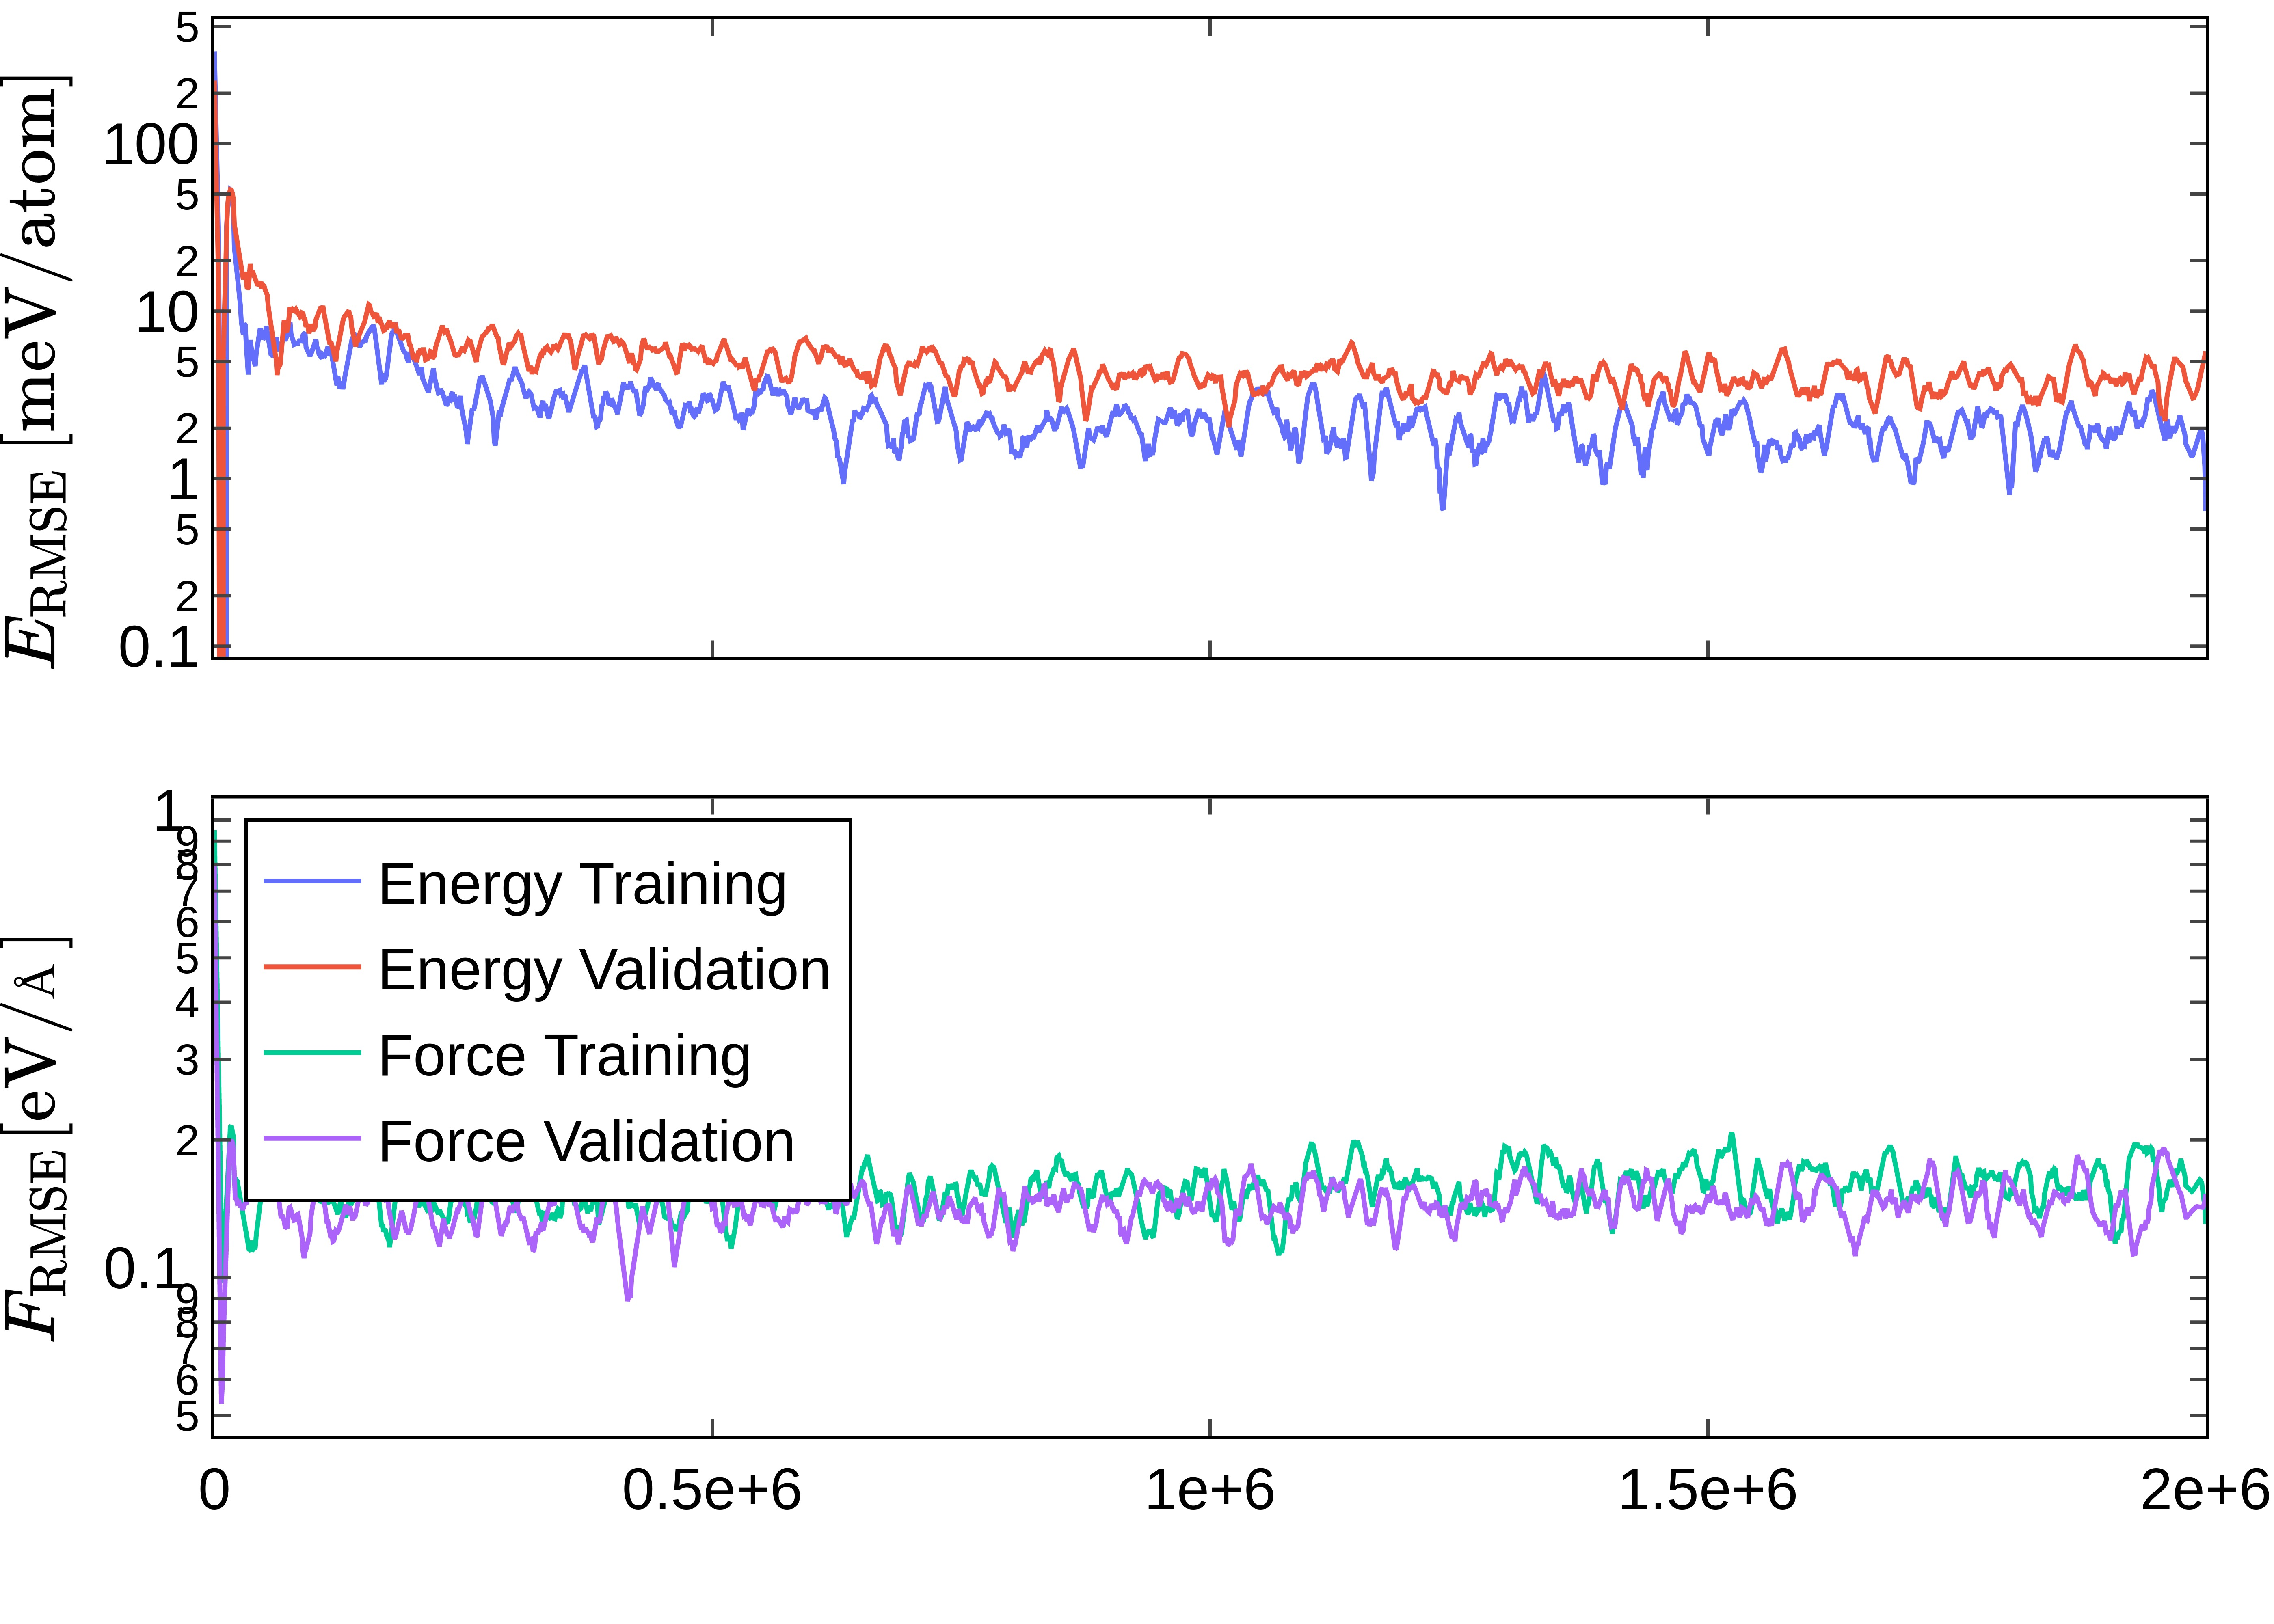
\includegraphics[width=.8\textwidth]{
      asset/crystalline_10,20,40d_10,10,10f_260222622s_energy_force_l_curve.jpg
    }
  \end{center}
  \caption{Learning curves for model \texttt{crystalline\_10,20,40d\_10,10,\allowbreak{}10f\_260222622s}.}
  \label{fig:crystalline_10,20,40d_10,10,10f_260222622s-learning-curves}
\end{figure}

\begin{figure}
  \begin{center}
    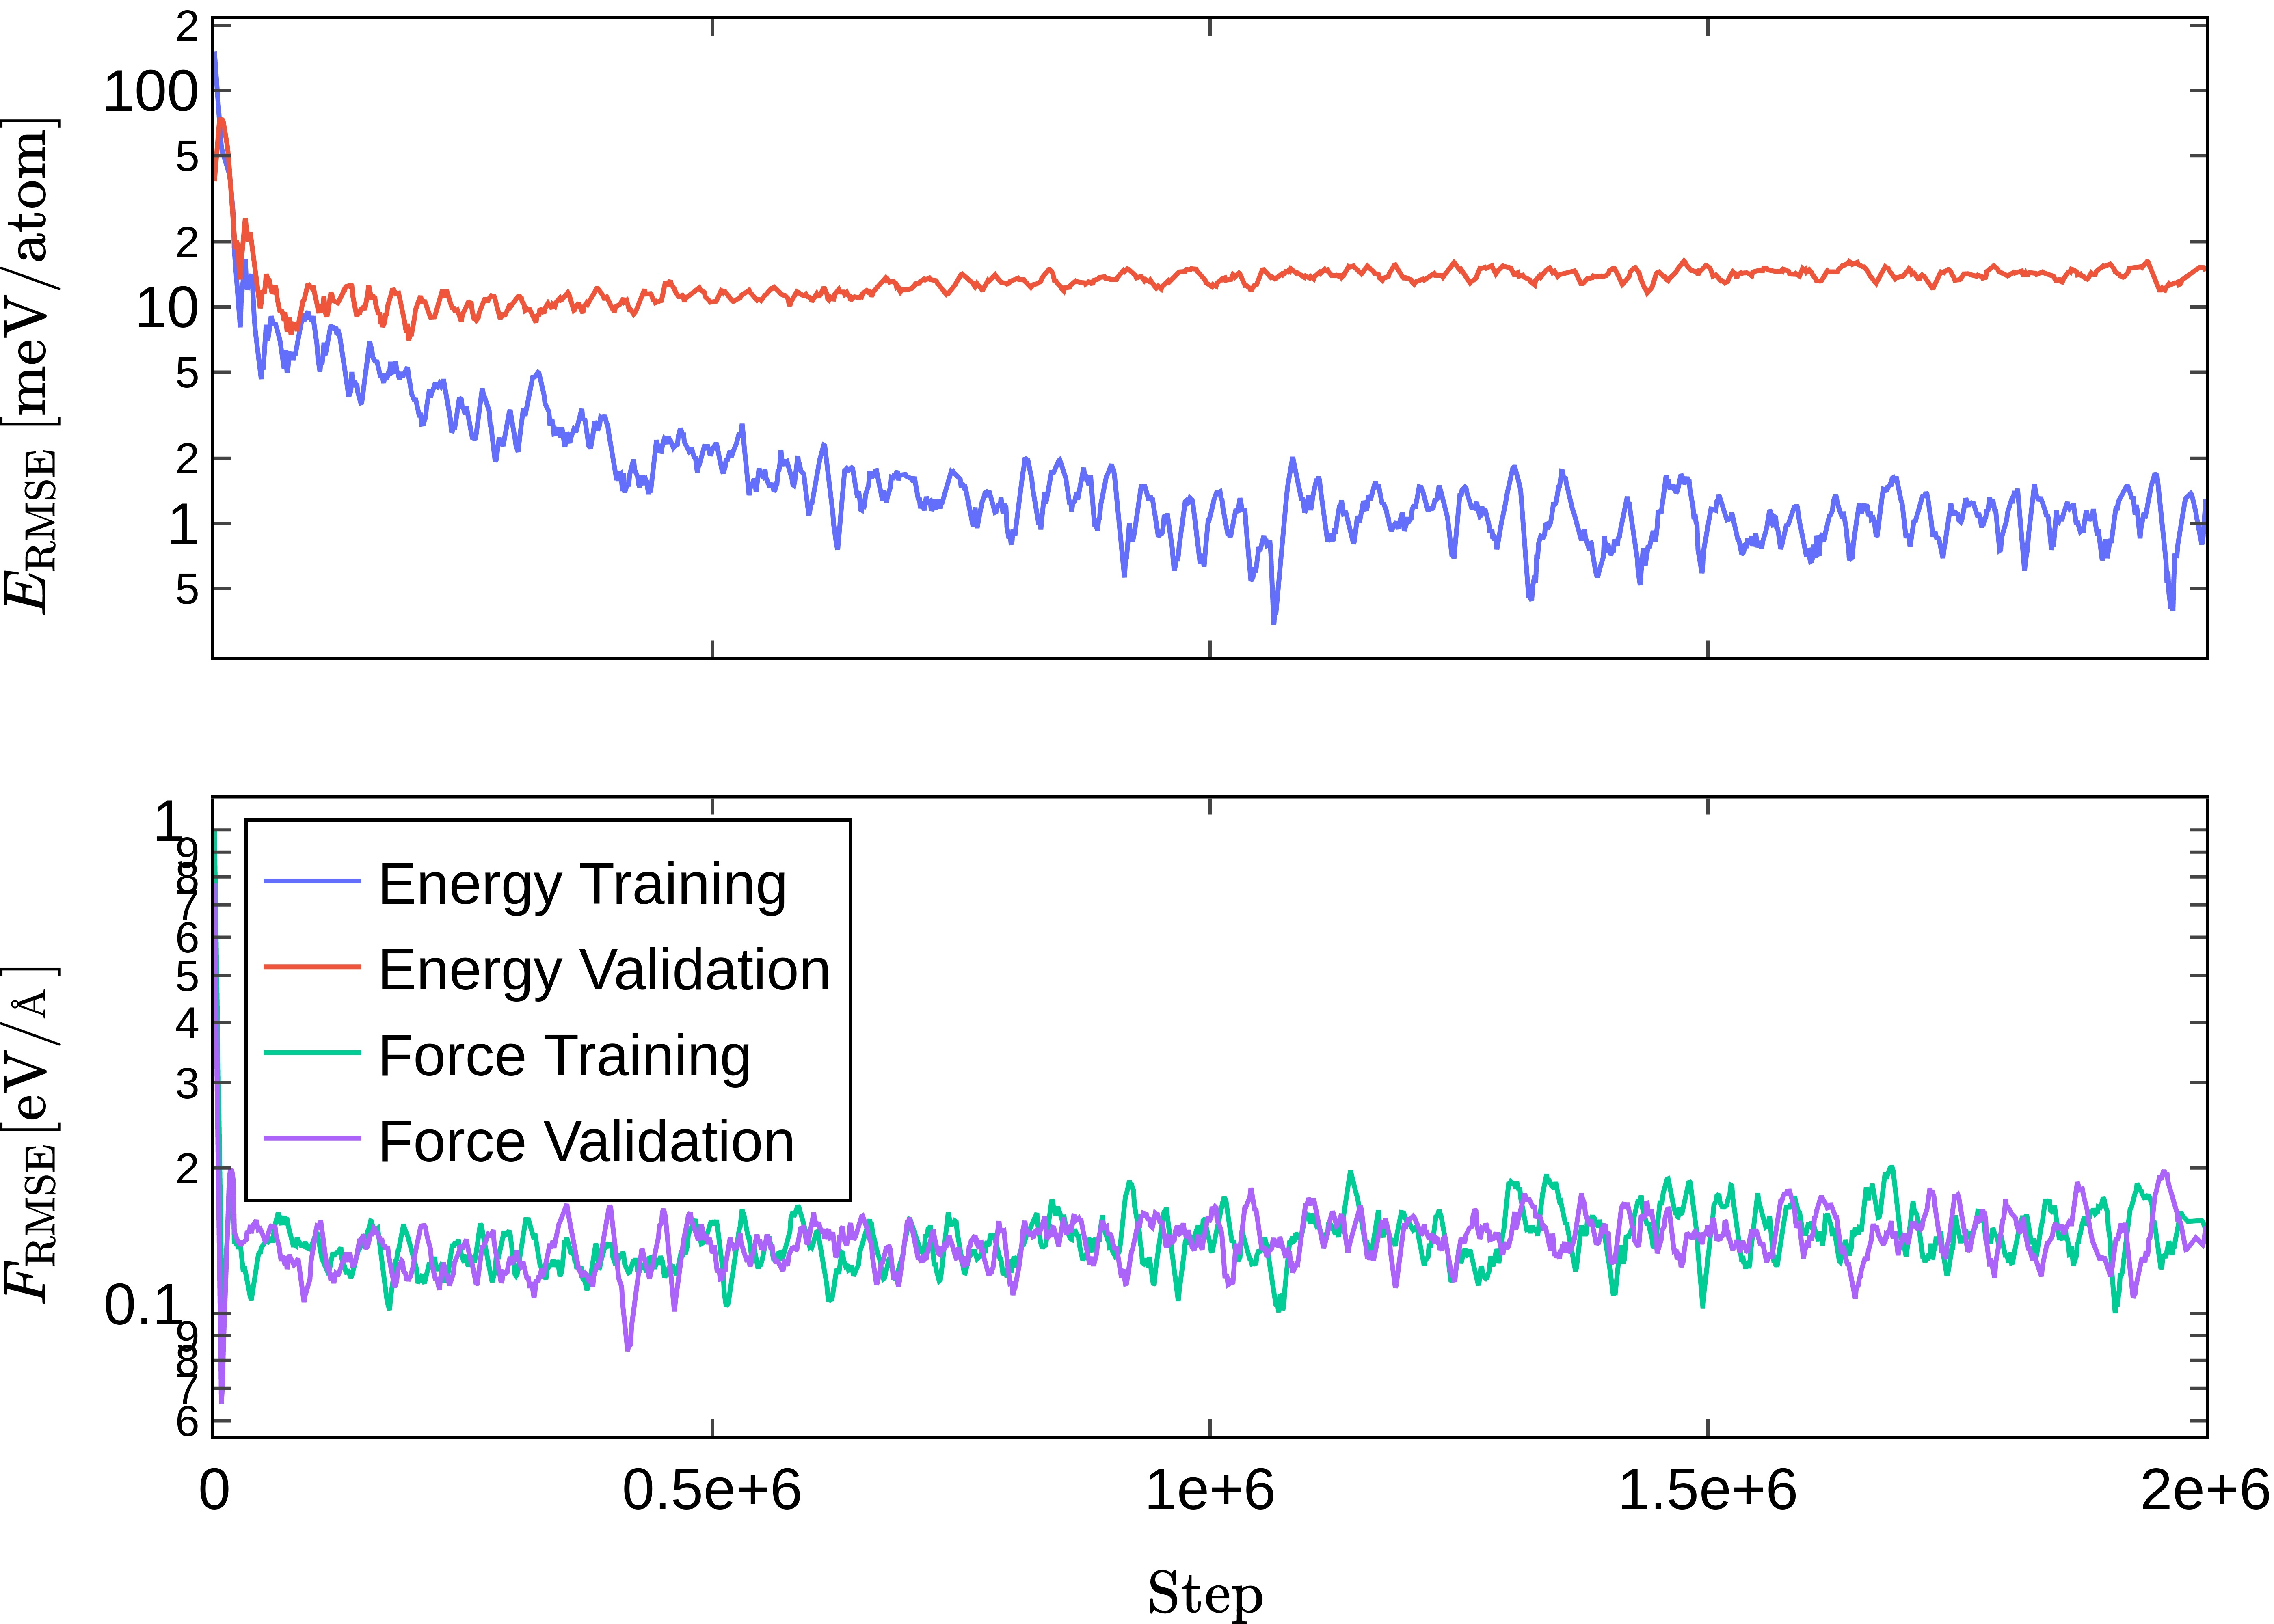
\includegraphics[width=.8\textwidth]{
      asset/crystalline_10,20,40d_75,75,75f_260222622s_energy_force_l_curve.jpg
    }
  \end{center}
  \caption{Learning curves for model \texttt{crystalline\_10,20,40d\_75,75,\allowbreak{}75f\_260222622s}.}
  \label{fig:crystalline_10,20,40d_75,75,75f_260222622s-learning-curves}
\end{figure}

\begin{figure}
  \begin{center}
    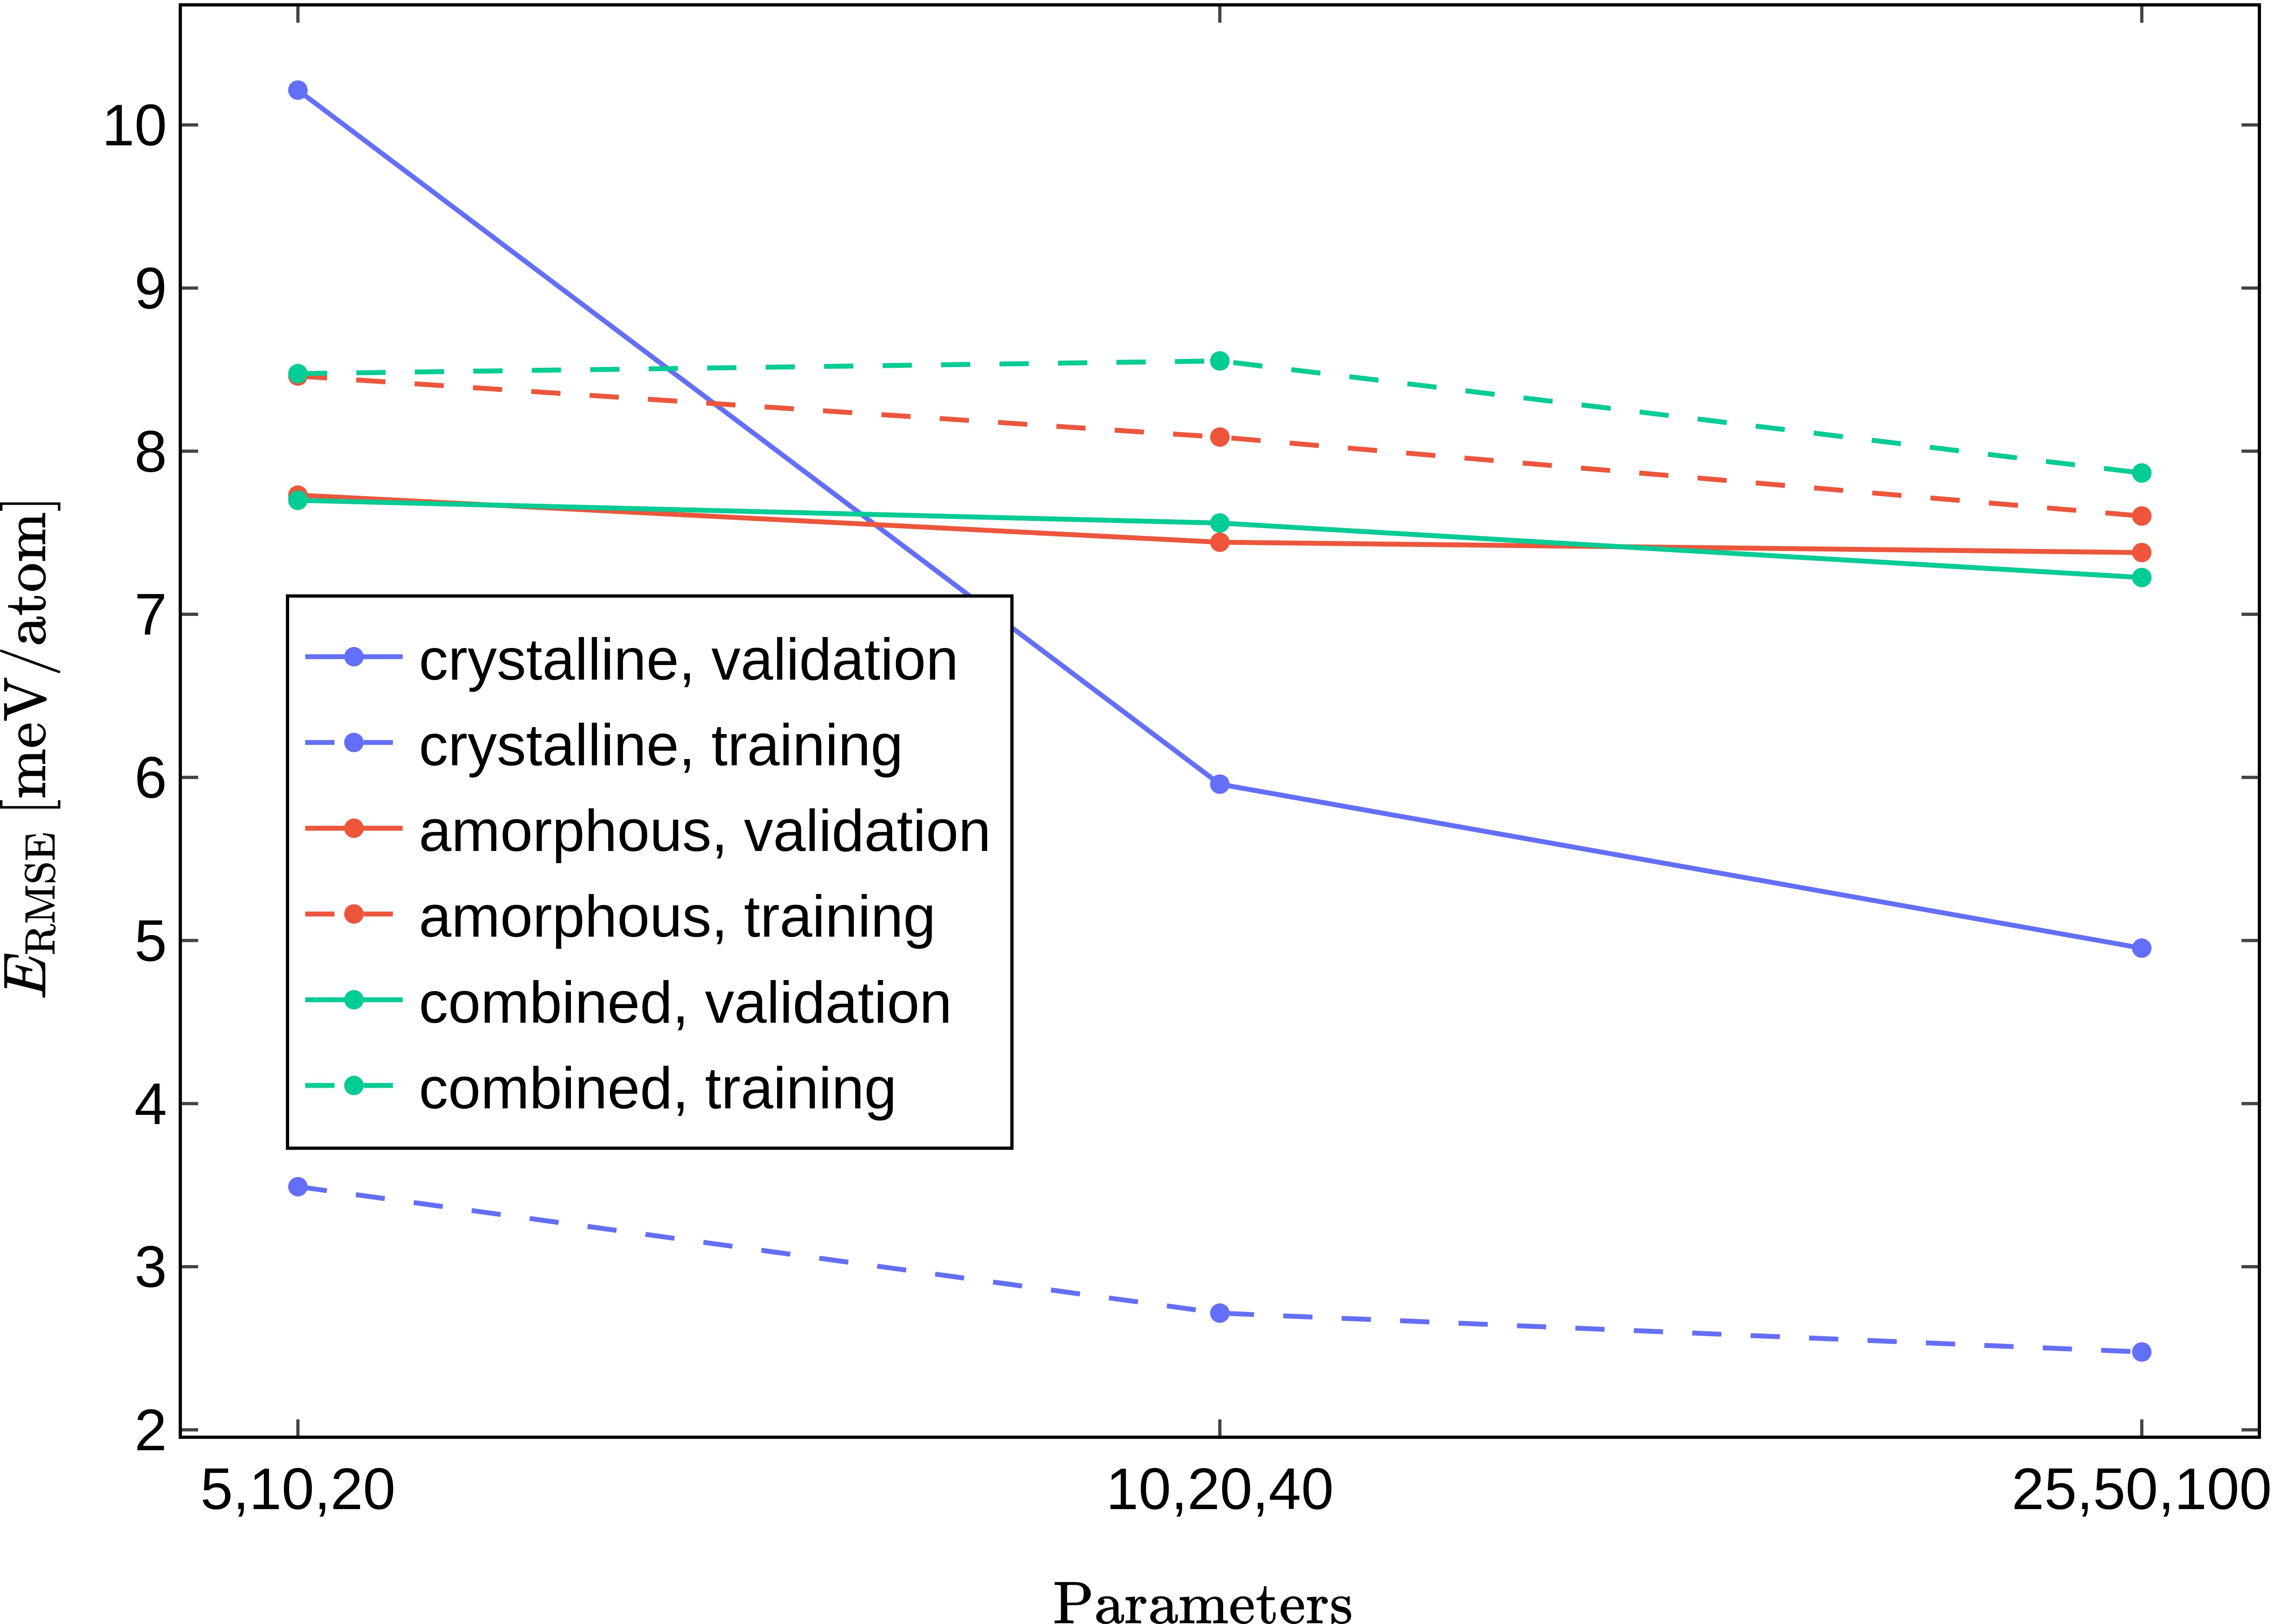
\includegraphics[width=.8\textwidth]{
      asset/descriptor_energy_error_evaluation.jpg
    }
  \end{center}
  \caption{Evaluation of energy errors for different descriptor neuron numbers.}
  \label{fig:descriptor_energy_error_evaluation}
\end{figure}

\begin{figure}
  \begin{center}
    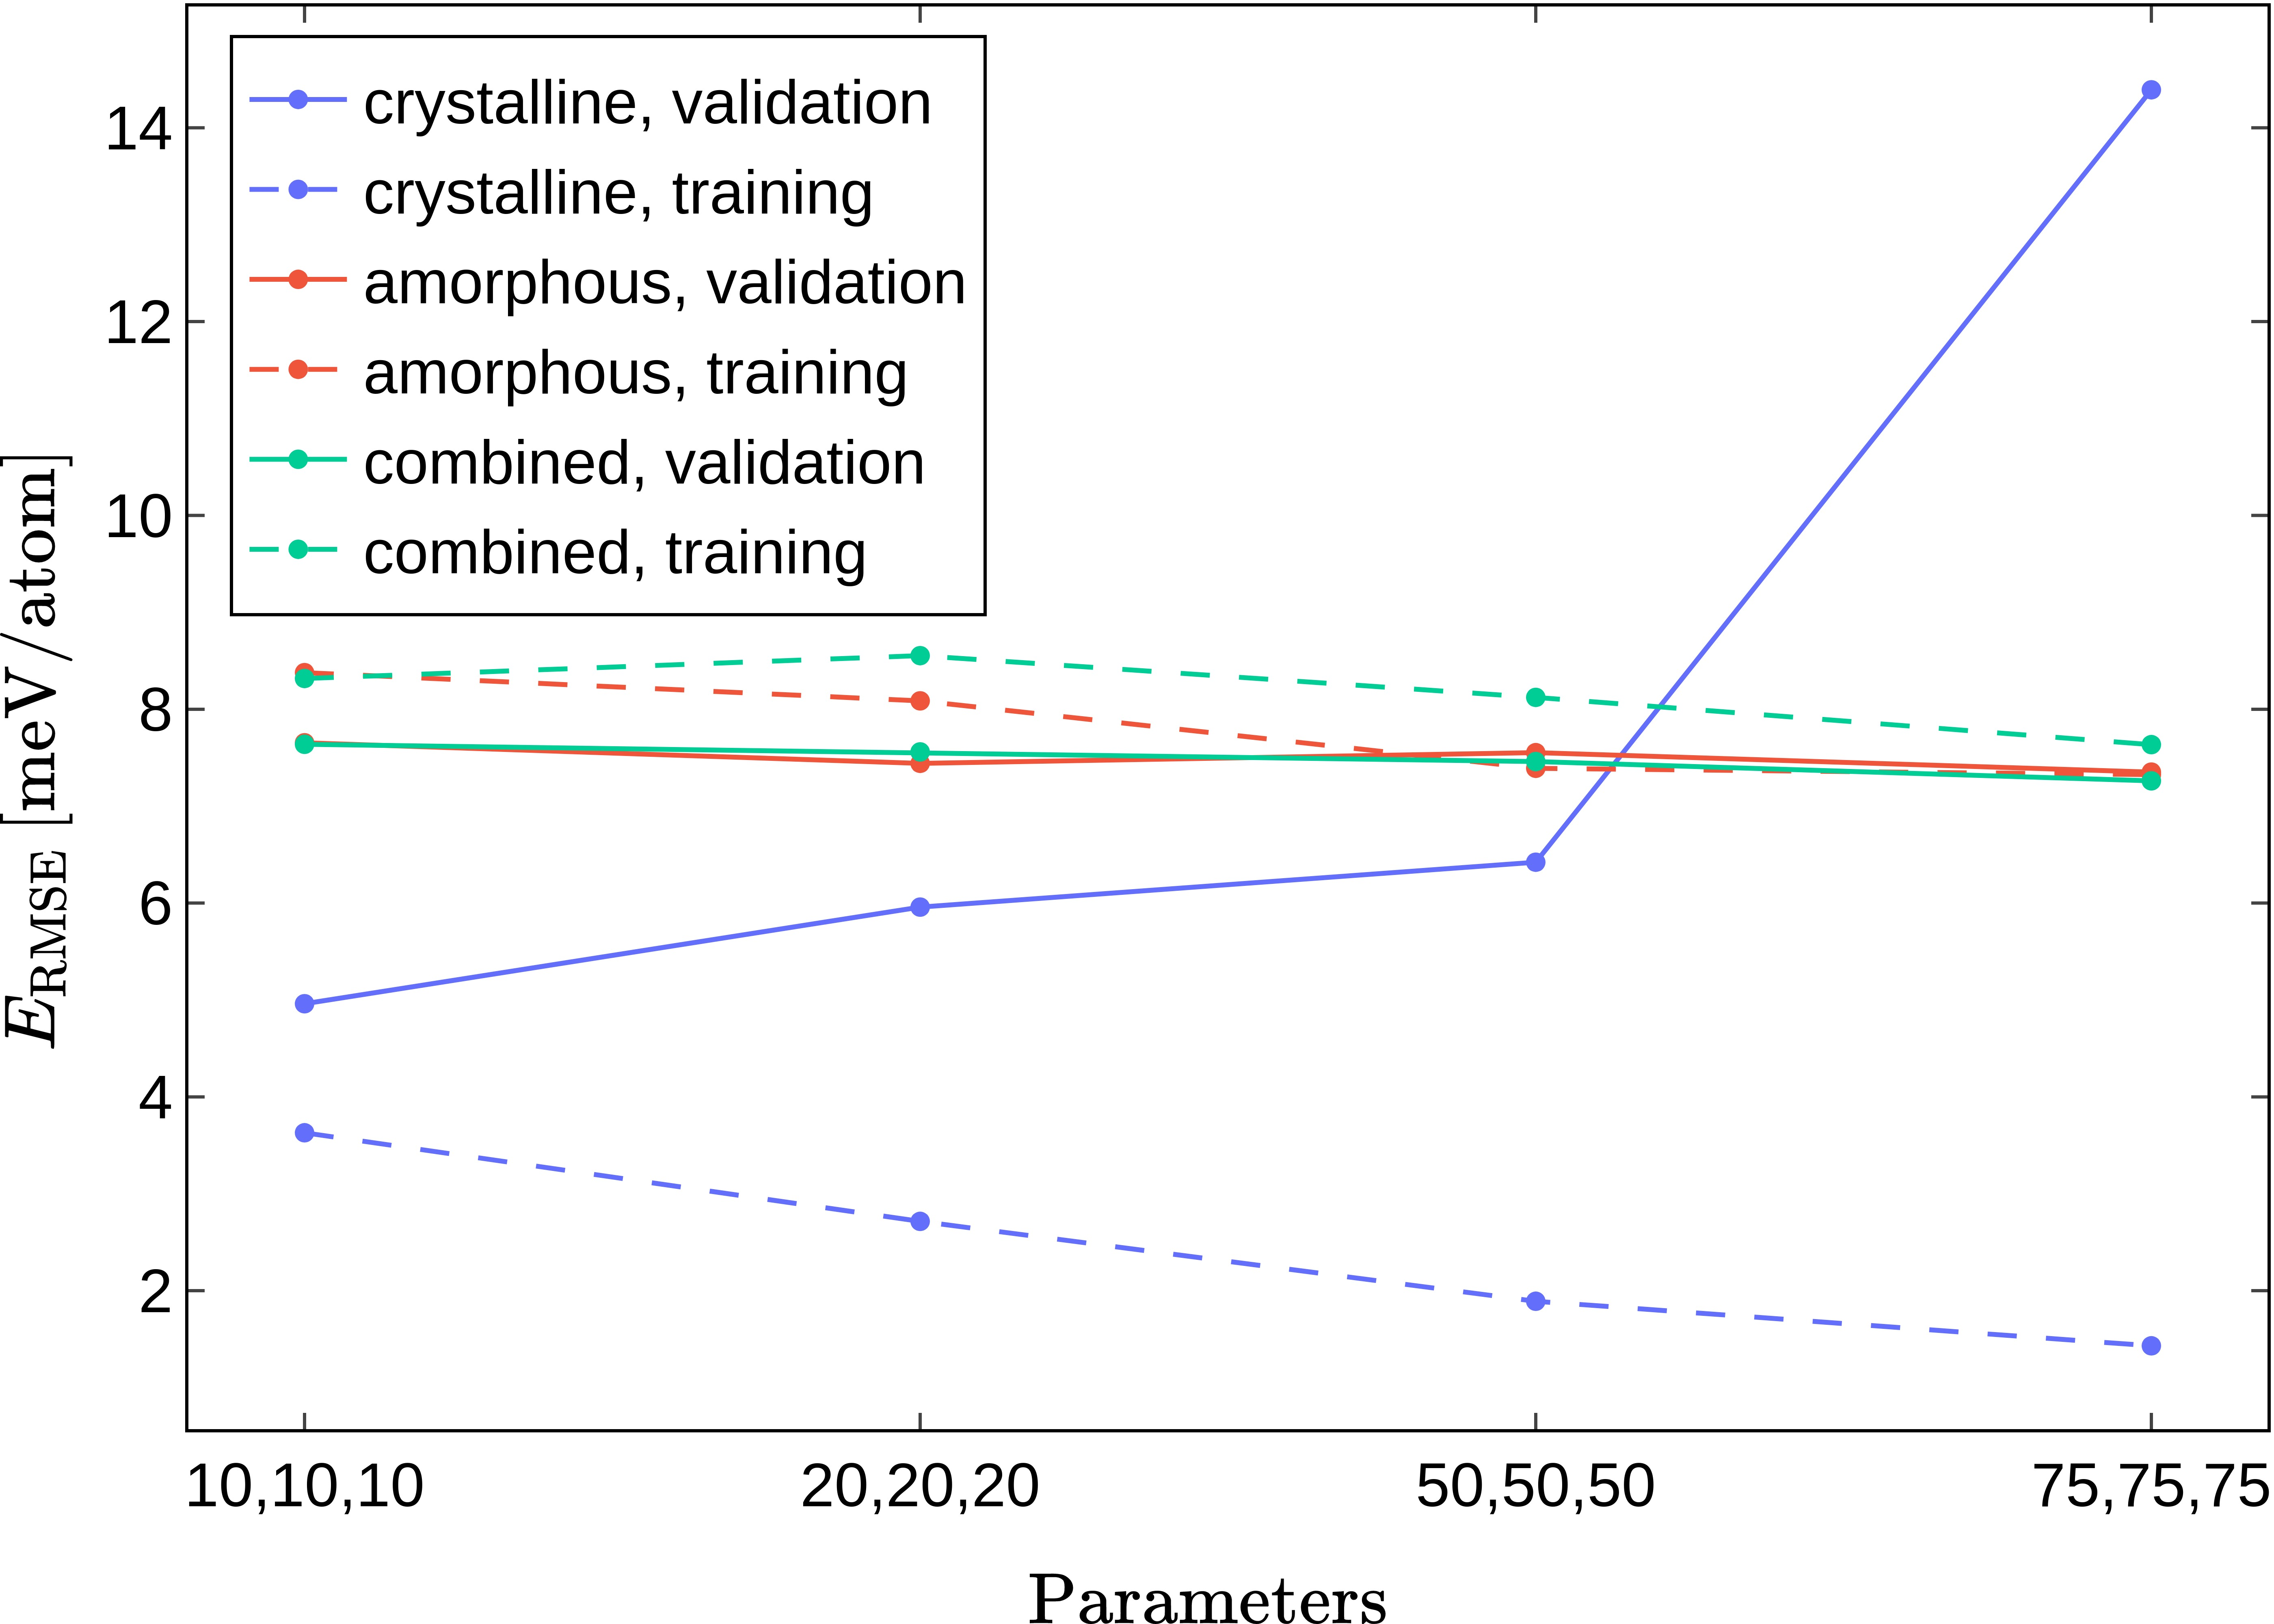
\includegraphics[width=.8\textwidth]{
      asset/fitting_energy_error_evaluation.jpg
    }
  \end{center}
  \caption{Evaluation of energy errors for different fitting neuron numbers.}
  \label{fig:fitting_energy_error_evaluation}
\end{figure}

\section{Inference Results}

The models \texttt{crystalline\_10,20,40d\_20,20,20f\_260222622s},
\texttt{cryst\-alline\_10,20,40d\_20,20,20f\_537693349s}, and
\texttt{crystalline\_10,20,\linebreak{}40d\_20,20,20f\_836424474s} were used to calculate
relaxation volume and bulk modulus for the Si diamond crystalline structure
at 0 K (cubic $\mathrm{F}\bar{\mathrm{d}}\mathrm{3m}$ space group). The
inference data with the fitted EOS models are shown below (figure
\ref{fig:crystalline_inference}). The calculated value for the relaxation
volume was $V_0 = 20.52 \pm 0.03$ \AA$^3$ and the calculated value for the
bulk modulus was
$B_{T_0} = 115 \pm 13 \, \mathrm{eV} \cdot \text{\AA}^{-3}$. Reference
materials for quantum mechanical calculations of the same structure give
values of $V_0 = 20.46$ \AA$^3$ and
$B_{T_0} = 98 \, \mathrm{GPa} \cdot \text{\AA}^{-3}$\cite{osti_1190959}.
Although the calculated values are not exactly in concordance with the
reference values, they are very close, and their relative errors are
only $\sim 0.3\%$ for the relaxation volume and $\sim 17 \%$ for the bulk
modulus. The values may differ firstly due to the different methodology and
configuration used for the qunatum mechanical calculations of the reference
and secondly due to the fact that the used models did not have enough training
data to converge exactly. Nonetheless, the results are very promising and show
that the models are able to predict the properties of the crystalline silicon
structure. This indicates a proper choice of the DNN hyperparameters. It is
also worth noting that the models were able to predict the properties of the
crystalline Si structure at 0 K even though they were only trained on data at
1500 K.

Comparing the inference results of the three models, it can be seen from the
figure \ref{fig:crystalline_inference} that the models give very similar
results near the equilibrium volume and start diverging significantly as more
strain is applied and the models are forced to extrapolate for unknown
conditions not seen in the learning data. To enhance the inference results,
more training data could be added for the volumes where the models diverge the
most.

\begin{figure}
  \begin{center}
    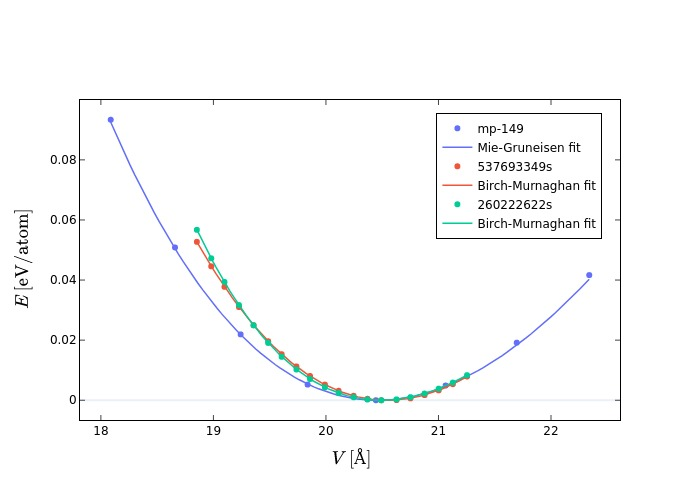
\includegraphics[width=.8\textwidth]{
      asset/crystalline_ev_curves.jpg
    }
  \end{center}
  \caption{Inference results for the Si diamond crystalline structure. The EV
  curves were shifted to have zero energy at the equilibrium volume for better
  comparison.}
  \label{fig:crystalline_inference}
\end{figure}

Next, the model \texttt{amorphous\_10,20,40d\_50,50,50f\_260222622s} was used
to calculate bulk modulus $B_0$ and volume thermal expansion coefficient
$\alpha_{V}$ for an amorphous silicon structure composed of 100 atoms with
density $\rho = 2.329 \, \mathrm{g} \cdot \mathrm{cm}^{-3}$. These material
properties were computed by fitting the Birch--Murnaghan EOS model to EV
curves calculated by the DNN at various temperatures. The results are shown in
figure \ref{fig:amorphous_inference}. The model seems to behave quite well at
temperatures up to 800 K. Above that temperature, the results start to produce
significant noise. Molecular dynamics at higher temperatures is more complex
and requires higher-quality predictions from the DNN to produce consistent
results. Most likely, our model is not able to produce such predictions
due to the low volume of the training data. Another reason could be that since
we only simulate 100 atoms in the amorphous structure, the statistical nature
of the simulation breaks down. These two problems could be solved by adding
more training data and simulating a larger number of atoms in the amorphous
structure. Another effect at play could be the fact that the amorphous Si
structure is not properly relaxed during the generation phase, as that would
require many more simulation steps. The structure is also being generated
using a different potential than the one used for the inference, which could
mean that even if the structure was properly relaxed, the relaxation state is
simply not compatible with the potential used for the inference. This could be
solved by using the same potential for both generation and inference and
by relaxing the structure for a longer time. Another problem could be that the
integration time used in the simulation is too large, which is also easily
solvable but would require more computational resources, which were not
available for this work.

\begin{figure}
  \begin{center}
    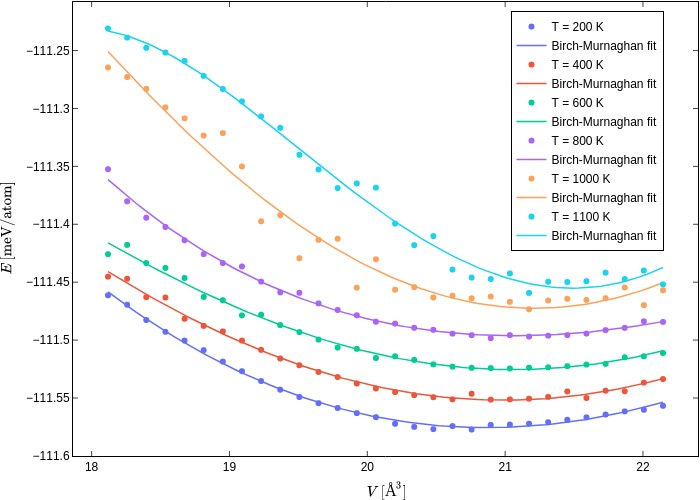
\includegraphics[width=.8\textwidth]{
      asset/amorphous_ev_curves.jpg
    }
  \end{center}
  \caption{Inference results for the Si amorphous structure at various
  temperatures.}
  \label{fig:amorphous_inference}
\end{figure}

\begin{figure}
  \begin{center}
    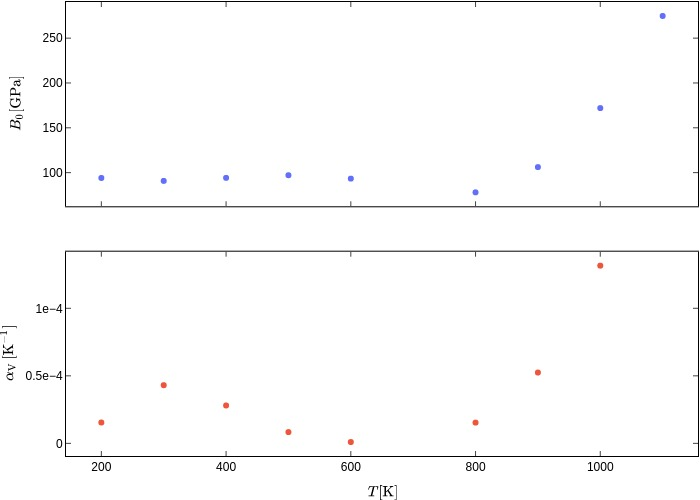
\includegraphics[width=.8\textwidth]{
      asset/amorphous_properties.jpg
    }
  \end{center}
  \caption{The dependence of the bulk modulus $B_0$ and volumetric thermal
  expansion coefficient $\alpha_V$ on temperature $T$ for the amorphous
  silicon structure.}
  \label{fig:amorphous_properties}
\end{figure}

Experimental values of the Young modulus $\mathcal{E}$ and the Poisson's ratio
$\nu$ for polycrystalline silicon material are $\sim 170 \, \mathrm{GPa}$ and
$\sim 0.22$, respectively \cite{Freund_Suresh_2003}. The relation between the
bulk modulus $B_0$, the Young modulus $\mathcal{E}$, and the Poisson's ratio
$\nu$ for an isotropic material is
\begin{equation}
  B_0 = \frac{\mathcal{E}}{3(1 - 2\nu)}.
\end{equation}
Using this formula, we can calculate the bulk modulus of polysilicon $B_0$ to
be $\sim 101 \, \mathrm{GPa}$. The modeled bulk modulus $B_0$ for the
amorphous silicon used in this work is
$\sim 94 \, \mathrm{GPa}$ at $T = 200 \, \mathrm{K}$,
$\sim 91 \, \mathrm{GPa}$ at $T = 300 \, \mathrm{K}$,
$\sim 94 \, \mathrm{GPa}$ at $T = 400 \, \mathrm{K}$,
and $\sim 78 \, \mathrm{GPa}$ at $T = 800 \, \mathrm{K}$.

The linear expansion coefficient $\beta$ for an amorphous Si is experimentally
measured to be $\sim 3.6 \cdot 10^{-6} \, \mathrm{K}^{-1}$ at
$T = 318.15 \, \mathrm{K}$, $\sim 3.0 \cdot 10^{-6} \, \mathrm{K}^{-1}$ at
$T = 418.15 \, \mathrm{K}$ \cite{TAKIMOTO2002314}. The relation between the
linear expansion coefficient $\beta$ and the volumetric expansion coefficient
$\alpha_V$ is
\begin{equation}
  \alpha_V = 3 \cdot \beta.
\end{equation}
Converting these values of the linear expansion coefficient $\beta$ to the
volumetric expansion coefficient $\alpha_V$ we get
$\sim 1.1 \cdot 10^{-5} \, \mathrm{K}^{-1}$ at $T = 318.15 \, \mathrm{K}$ and
$\sim 0.9 \cdot 10^{-5} \, \mathrm{K}^{-1}$ at $T = 418.15 \, \mathrm{K}$.
Our models arrived at values for $\alpha_V$ to be
$\sim 4.3 \cdot 10^{-5} \, \mathrm{K}^{-1}$ at
$T = 350 \, \mathrm{K}$, $\sim 2.8 \cdot 10^{-5} \, \mathrm{K}^{-1}$ at
$T = 450 \, \mathrm{K}$. The inference results for the bulk modulus $B_0$ had
relative errors of $\sim 10 \%$ and their quality was on par with the quality
of the inference results for the crystalline silicon except for outliers
($T = 700 \, \mathrm{K}$) and for too high temperatures
($T > 800 \, \mathrm{K}$). The results for the volumetric thermal expansion
coefficient unfortunately ended with significant relative errors of
$\sim 290 \%$. The very high relative errors for the volumetric
thermal expansion coefficient $\alpha_V$ are most likely caused by the fact
that the calculations depend mostly on correct predictions of the relaxation
volume $V_0$ of the amorphous structure at various temperatures. Even though
the DNN models were able to predict the volume $V_0$ of the crystalline
structure very well, the predictions for the amorphous structure are by nature
more uncertain as they depend on proper relaxation of the generated structure
and are thus sensitive to the choice of the potentials used in the
various steps of the computation process (OpenMX pseudopotentials used for
the training data generation, OpenKIM potentials used for the amorphous
structure generation and relaxation, and the DeepMD potential itself used for
the MD simulation). Furthermore, as has already been mentioned, the size of
the amorphous structure used in the inference is relatively small, which
breaks the statistical nature of the system and causes the results to be noisy
at higher temperatures. It's also obvious that the results for the $\alpha_V$
are much more error-prone than the results for the $B_0$ as the former is
calculated from just one value (the volume $V_0$) while the latter is given by
the slope of the EV curve, which is much more resilient to noise. These errors
are, however, just a rough estimate, as the experimental values for the
amorphous silicon are obtained for vastly different conditions (the material
is not completely amorphous but polycrystalline, the temperatures and
pressures are different, the measurement methods are different, etc.) than the
ones calculated in this work. The calculated values are more uncertain the
higher the temperature is, as can be clearly seen from the noise in the EV
curves for higher temperatures in figure \ref{fig:amorphous_inference}. This
is expected, as the molecular dynamics is more complicated at higher
temperatures and the DNN models are forced to extrapolate more. The results
are nonetheless very promising and show that the models are able to predict
the properties of the amorphous silicon structure.
